\chapter{模型和变换矩阵}
本章中的大多数宝石都与变换有关:如何组合、分解和操作它们。第一个Gem描述了如何使用四元数表示在两个方向之间进行插值,并在插值的末尾添加了额外的自旋。第五个Gem是第一个的有用伴侣,因为它讨论了与插值发生时的转换选择有关的问题。第七篇Gem描述了一种替代的插值技术,使用B\'ezier曲线。

第二个和第三个gem讨论了如何将复杂的转换分解为更简单的组件。本节中的第四个和第六个Gems描述了产生旋转的两种互补技术,它们在某种意义上是随机的,并且在方向上均匀分布。这些宝石是对以前的宝石的改进。

本节中的最后一个Gem是征求意见稿,为那些对基于物理的建模感兴趣的人提供了有用的信息。本文给出了超二次椭球和环面体积和质量性质的封闭形式表达式,并讨论了惯性张量的计算和使用。

\newpage
\section{带有额外自旋的四元数插值}
\begin{center}
\small{
Jack Morrison\\
Digital Insight\\
Evergreen, Colorado}
\end{center}

Quaternions are handy for representing the orientation or rotation of a 3-D object (Shoemake, 1985). The "Slerp" operation (spherical linear interpolation) interpolates between two quaternions at a constant speed, using the most direct rotational path between the orientations. An animator may, however, want the interpolation to provide extra spins along the same path (complete revolutions about the same axis-see Fig. 1). This Gem gives a simple formula for doing this, derived with the help of Steven Gabriel.

Given two unit quaternions $\mathbf{A}$ and $\mathbf{B}$, and an interpolation parameter $\alpha$ ranging from 0 to 1 , the basic Slerp equation is

$$
\operatorname{Slerp}(\mathbf{A}, \mathbf{B} ; \alpha)=\mathbf{A}\left(\mathbf{A}^{-1} \mathbf{B}\right)^{\alpha} .
$$

An easier-to-implement equation uses the angle $\theta$ between the quaternions:

$$
\begin{aligned}
\theta &=\operatorname{acos}(\mathbf{A} \cdot \mathbf{B}) \\
\operatorname{Slerp}(\mathbf{A}, \mathbf{B} ; \alpha) &=\frac{\sin (\theta-\alpha \theta)}{\sin \theta} \mathbf{A}+\frac{\sin (\alpha \theta)}{\sin \theta} \mathbf{B} .
\end{aligned}
$$

To include $\mathrm{k}$ additional spins, determine

$$
\varphi=\theta+\mathrm{k} \pi,
$$


\begin{center}
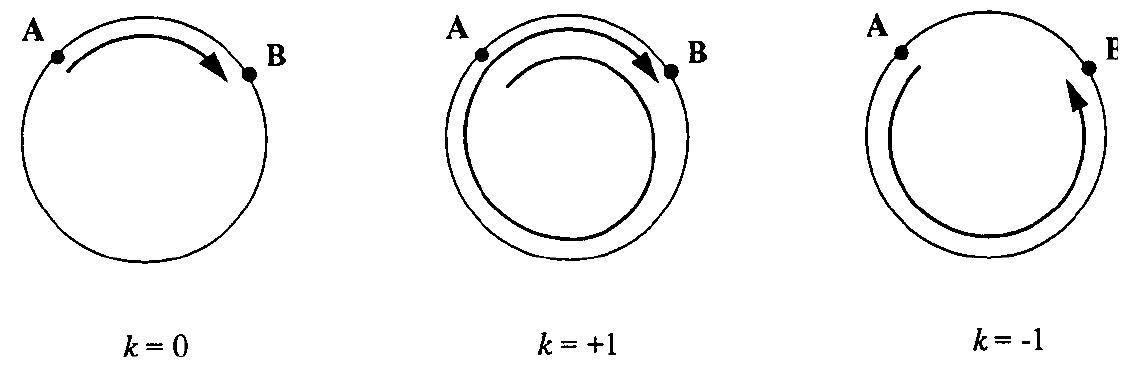
\includegraphics[max width=\textwidth]{2022_11_30_0cbb01a33d99487fc27fg-129}
\end{center}

Figure 1. Slerp (A, B) with $\mathrm{k}$ additional spins.

then

$$
\operatorname{Slerp}(\mathbf{A}, \mathbf{B}, \mathrm{k} ; \boldsymbol{\alpha})=\frac{\sin (\theta-\alpha \varphi)}{\sin \theta} \mathbf{A}+\frac{\sin (\alpha \varphi)}{\sin \theta} \mathbf{B}
$$

Figure 1 shows the effect of $\mathrm{k}$, viewing orientations $\mathbf{A}$ and $\mathbf{B}$ along the rotation axis. For $\mathrm{k}=0$, $\mathrm{f}$ equals $\mathrm{q}$, the equation reduces to the original form, and the interpolation follows the shortest circular path from A to $\mathbf{B}$. For $\mathrm{k}=+1$, one full additional rotation is generated as a goes from 0 to 1. For $\mathrm{k}=-1$, the interpolation goes the "long" way around.

The C implementation first checks if $\mathbf{A}$ and $\mathbf{B}$ are on opposite hemispheres $(\cos \theta<0$ ). If so, the interpolation is modified to use the negation of B (which represents the same orientation as B itself), to ensure that the shortest rotation path is taken. It also checks whether A and $\mathbf{B}$ are the same, so that $\sin \theta=0$, and no axis is defined for spinning. If $\mathbf{A}$ and $\mathbf{B}$ represent orientations 180 degrees apart, all rotation paths are the same length, but the quaternions still define an axis for spinning. Note that for a given $\mathbf{A}, \mathbf{B}$, and $\mathrm{k}$, the quantities $\theta, \varphi$, and $\sin \theta$ could be computed once outside the interpolation loop for efficiency.

See also G1, 498.\\
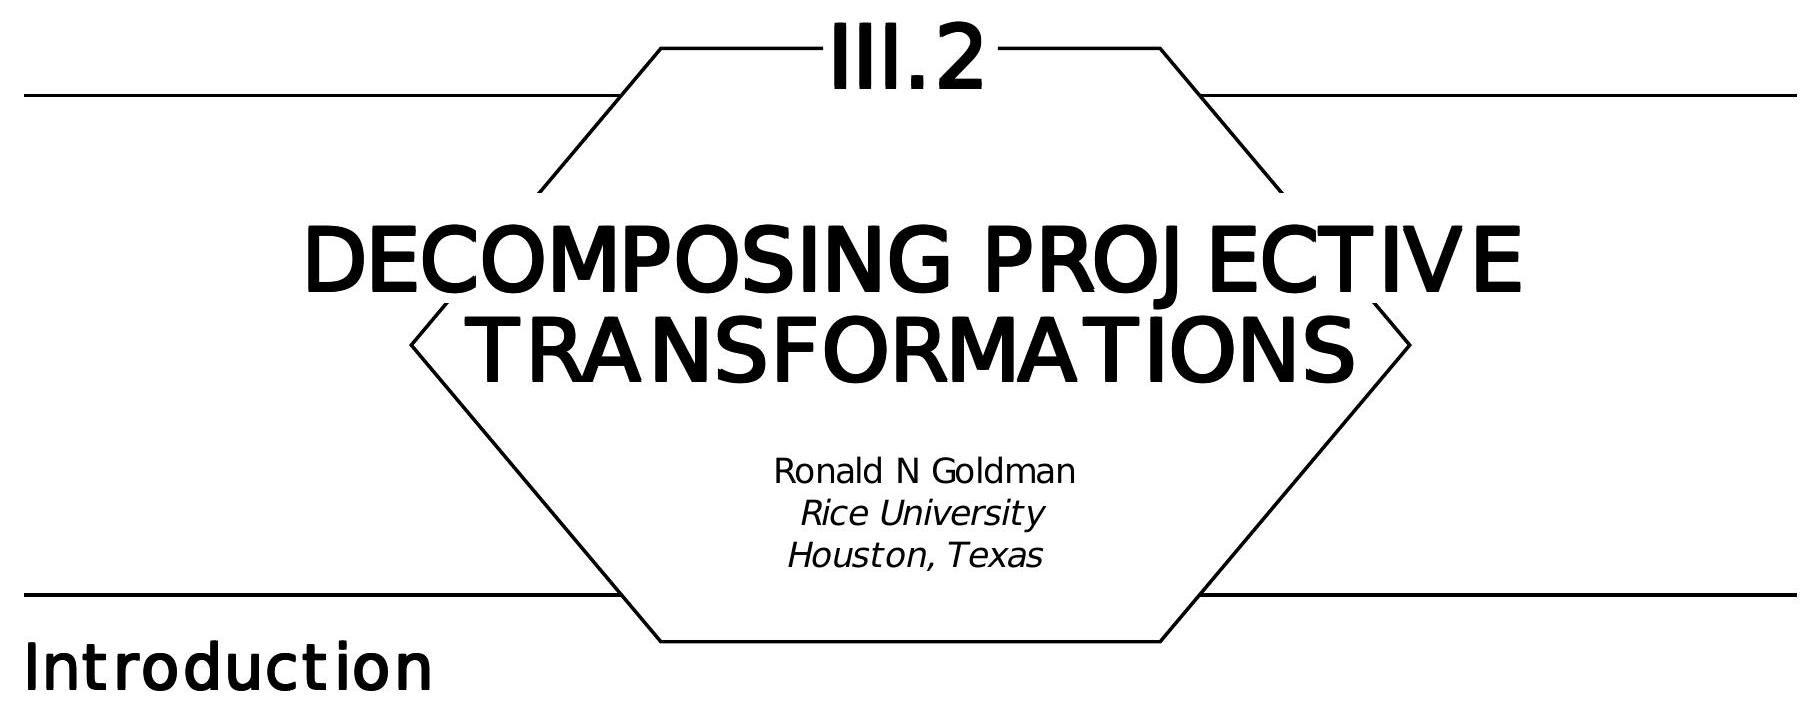
\includegraphics[max width=\textwidth, center]{2022_11_30_0cbb01a33d99487fc27fg-130}

In another Gem (III.3) we show how to decompose linear and affine transformations of three-dimensional space into the products of scale, shears, rotations, translations, and projections. The goal of this gem is to demonstrate how to decompose an arbitrary projective transformation of three-dimensional space into simple, geometrically meaningful factors. For an alternative approach, see Thomas (1991).

Let us begin by recalling the difference between linear, affine, and projective transformations. Consider a point $\mathrm{P}$ with coordinates $(\mathrm{x}, \mathrm{y}, \mathrm{z})$, and let $\mathrm{P}_{\text {new }}$ with coordinates $\left(\mathrm{x}_{\text {new }}, \mathrm{y}_{\text {new }}, \mathrm{z}_{\text {new }}\right.$ ) denote the new transformed point. Formulas that express the new coordinates $\mathrm{x}_{\text {new }}, \mathrm{y}_{\text {new }}, \mathrm{z}_{\text {new }}$ in terms of the original coordinates $\mathrm{x}, \mathrm{y}, \mathrm{z}$ are given by the following equations:

Linear:

Affine:

Projective:

$$
\begin{aligned}
&\mathrm{x}_{\text {new }}=a x+b y+c z, \\
&x_{\text {new }}=a x+b y+c z+d, \\
&x_{\text {new }}=(a x+b y+c z+d) /(\alpha x+\beta y+\gamma z+\delta),
\end{aligned}
$$

with analogous formulas for $\mathrm{y}_{\text {new }}$ and $\mathrm{z}_{\text {new }}$. Remember, too, that for projective transformations, the denominators of $\mathrm{x}_{\text {new }} \mathrm{y}_{\text {new }}, \mathrm{z}_{\text {new }}$ are identical.

Linear transformations are usually represented by $3 \mathrm{X} 3$ matrices $\mathrm{L}$. A point $\mathrm{P}=(\mathrm{x}, \mathrm{y}, \mathrm{z})$ transforms according to the formula

$$
\mathrm{P}_{\text {new }}=\mathrm{P} * \mathrm{~L} \text {, }
$$

\section{III.2 DECOMPOSING PROJ ECTIVE TRANSFORMATIONS}
where $*$ denotes matrix multiplication. Similarly, affine transformations are represented by $4 \times 3$ matrices

$$
\mathrm{A}=\mid \begin{aligned}
&\mathrm{L} \\
&\mathrm{T}
\end{aligned} .
$$

Here the upper $3 \times 3$ submatrix L represents a linear transformation and the last row $\mathrm{T}$ represents a translation. Let $\mathrm{P}^{*}=(\mathrm{P}, 1)$. Then a point $\mathrm{P}$ transforms according to the formula

$$
\mathrm{P}_{\text {new }}=\mathrm{P} * * \mathrm{~A}=\mathrm{P} * \mathrm{~L}+\mathrm{T}
$$

Projective transformations can be represented by $4 \times 4$ matrices

$$
\mathbf{M}=\left|\begin{array}{cc}
\mathrm{L} & \mathrm{N}^{\mathrm{t}} \\
\mathrm{T} & \mathrm{d}
\end{array}\right|,
$$

where the upper $3 \times 3$ submatrix $L$ represents a linear transformation, the vector $\mathrm{T}$ represents a translation, and the column $(\mathrm{N} d)^{\mathrm{t}}$ (the superscript $t$ denotes transpose) represents the projection. A homogeneous point $\mathrm{P}^{*}=(\mathrm{P}, 1)$ transforms according to the formula

$$
\mathrm{P}_{\text {new }}=\mathrm{P} * * \mathrm{M}=(\mathrm{P} * * \mathrm{~A}) /(\mathrm{P} \cdot \mathrm{N}+\mathrm{d})=(\mathrm{P} * \mathrm{~L}+\mathrm{T}) /(\mathrm{P} \cdot \mathrm{N}+\mathrm{d}) \text {, }
$$

where by convention $(\mathrm{x}, \mathrm{y}, \mathrm{z}, \mathrm{w})=(\mathrm{x} / \mathrm{w}, \mathrm{y} / \mathrm{w}, \mathrm{z} / \mathrm{w})$. That is, by convention, after performing the matrix multiplication, we divide by the homogeneous coordinate $\mathrm{w}_{\text {new }}$ to recover the actual point. Projective transformations are very important in computer graphics because perspective is a projective transformation (Goldman, 1990).

\section{First Decomposition Algorithm-Perspective in Four Dimensions}
The standard way to factor any projective transformation of three-dimensional space is first to embed three-space into four-space, next to apply the $4 \times 4$ matrix $M$ as a linear transformation in four-space, then to

\section{III.2 DECOMPOSING PROJ ECTIVE TRANSFORMATIONS}
apply a perspective projection of four-space with the eye point at the origin and the perspective hyperplane at $\mathrm{w}=1$, and finally to project from four-space back to three-space by identifying the four-dimensional hyperplane $\mathrm{w}=1$ with standard three-dimensional space. That is, we map

$$
\mathrm{R}^{3} \rightarrow \mathrm{R}^{4} \rightarrow \mathrm{R}^{4} \rightarrow \mathrm{R}^{3}
$$

by sending

$$
\mathrm{P} \rightarrow \mathrm{P}^{*}=(\mathrm{P}, 1) \rightarrow \mathrm{Q}^{*}=(\mathrm{Q}, 1)=(\mathrm{P}, 1) * \mathrm{M} * \mathrm{G} \rightarrow \mathrm{Q},
$$

where $G$ is the perspective transformation of $R^{4}$ from the origin into the hyperplane $\mathrm{w}=1$.

From the point of view of computer graphics and geometric modeling, this decomposition is not very satisfactory. To complete this decomposition, we would need to factor an arbitrary transformation M of four-dimensional space into simple, geometrically meaningful, fourdimensional transformations. While it is possible to do so, this violates the spirit of what we are trying to accomplish. In computer graphics and geometric modeling, we generally apply modeling transformations to position an object in space, and then apply a perspective projection to position the object on the screen for viewing. All these transformations occur in three dimensions so we should never really need to discuss transformations of higher-dimensional space. It is these three-dimensional transformations that we would like to recapture in our decomposition of an arbitrary projective transformation.

\section{Second Decomposition Algorithm Affine $*$ Projective}
To obtain a better decomposition, we can factor any projective transformation by using the product formula

$$
\left|\begin{array}{cc}
\mathrm{L} & \mathrm{N}^{\mathrm{t}} \\
\mathrm{T} & \mathrm{d}
\end{array}\right|=\left|\begin{array}{cc}
\mathrm{L} & 0 \\
\mathrm{~T} & 1
\end{array}\right| *\left|\begin{array}{cc}
\mathrm{I} & \Omega^{\mathrm{t}} \\
0 & \mathrm{~d}-\mathrm{T} * \Omega^{\mathrm{t}}
\end{array}\right|,
$$

\section{III.2 DECOMPOSING PROJ ECTIVE TRANSFORMATIONS}
where $\mathrm{L} * \Omega^{\mathrm{t}}=\mathrm{N}^{\mathrm{t}}$ This factoring certainly works when $\mathrm{L}$ is nonsingular, since then we can simply take $\Omega=N *\left(\mathrm{~L}^{-1}\right)^{\mathrm{t}}$, but it also works even if $\mathrm{L}$ is singular provided only that $\mathrm{N}$ is in the image of $\mathrm{L}^{\mathrm{t}}$. Now the first factor is simply the affine transformation given by the linear transformation L followed by the translation $\mathrm{T}$, and the second factor is a pure projective transformation. We know from Gem III.3 how to factor any affine transformation of three-dimensional space into simple, geometrically meaningful factors. Thus, if $\mathrm{N}$ is in the image of $\mathrm{L}^{\mathrm{t}}$, we can use this product formula to decompose a projective transformation into simple, geometrically meaningful factors, followed by a pure projective transformation.

What is the effect of the pure projective transformation? Consider the pure projective transformation matrix

$$
\mathrm{M}^{*}=\left|\begin{array}{cc}
\mathrm{I} & \Omega^{\mathrm{t}} \\
0 & \mathrm{~d}^{*}
\end{array}\right| .
$$

By convention, $\mathrm{M}^{*}$ transforms a point according to the formula

$$
P_{\text {new }}=P /\left(P \cdot \Omega+d^{*}\right) \text {. }
$$

Thus, any point $\mathrm{P}$ satisfying the equation

$$
P \cdot \Omega+d^{*}=1
$$

is left invariant by the transformation $\mathrm{M}^{*}$. But this equation is linear, so it defines a plane. Thus, the projective transformation $\mathrm{M}^{*}$ leaves a plane of points unmoved. Moreover, if $S$ is the plane defined by the linear equation

$$
P \cdot \Omega+d^{*}=0
$$

then $\mathrm{M}^{*}$ maps $\mathrm{S}$ to infinity. Finally, for an arbitrary point $\mathrm{P}$

$$
(P \cdot \Omega+d *)=\text { signed distance to the plane } S .
$$

Thus, the pure projective transformation $\mathrm{M}^{*}$ maps planes at a fixed

\section{III.2 DECOMPOSING PROJ ECTIVE TRANSFORMATIONS}
distance from $\mathrm{S}$ into other planes at a new fixed distance from S. Note, too, that the plane at infinity $(\mathrm{w}=0)$ is mapped to a finite plane.

From the perspective of computer graphics and geometric modeling, this decomposition of an arbitrary projective transformation into the product of a purely affine and a purely projective transformation is still not entirely satisfactory. In computer graphics, affine modeling transformations are usually followed by perspective projections. Thus, we would like, whenever possible, to factor a projective transformation into the product of an affine transformation and a perspective projection.

In one special case we do actually achieve this goal. Observe that if $\mathrm{d}^{*}=0$, then $\mathrm{P}_{\text {new }} \cdot \Omega=1$. Thus, $\mathrm{P}_{\text {new }}$ always lies on the invariant plane of $\mathrm{M}^{*}$. In this case, $\mathrm{M}^{*}$ is actually a perspective projection with the eyepoint at the origin and the perspective plane given by the linear equation $\mathrm{P} \cdot \Omega=1$. Thus, if $\mathrm{N}^{\mathrm{t}}=\mathrm{L} * \Omega^{\mathrm{t}}$ (that is, if $\mathrm{N}$ is in the image of $\mathrm{L}^{\mathrm{t}}$, e.g., $\mathrm{L}$ is nonsingular) and $\mathrm{d}=* \Omega^{\mathrm{t}}$, then our product formula actually give us the decomposition that we desire, since the second factor is a perspective projection. More generally, we need to decide when a projective transformation $\mathrm{M}$ has a perspective factor $\mathrm{M}^{*}$. One hint we can apply here is that if $d^{*}=0$, then $\operatorname{Det}\left(\mathrm{M}^{*}\right)=0$.

\section{Third Decomposition Algorithm- Perspective $*$ Affine}
If a projective transformation has a perspective factor, then it must be a singular matrix. This is easy to see because every perspective transformation M has an eyepoint E that is mapped to a singularity-that is, to the point with homogeneous coordinates $(0,0,0,0)$. Thus,

$$
\mathrm{E} * \mathrm{M}=0 \text {, }
$$

so the eyepoint $\mathrm{E}$ is an eigenvector of the matrix $M$ corresponding to the eigenvalue 0 . Thus, $M$ must be singular. We shall show that if $L$ is nonsingular, then the converse is also true. That is, if $\mathrm{M}$ is a singular $4 \times 4$ matrix whose upper $3 \times 3$ submatrix L is nonsingular, then M can be factored into the product of a perspective projection and an affine transformation.

\section{III.2 DECOMPOSING PROJ ECTIVE TRANSFORMATIONS}
Suppose, then, that we have a singular $4 \times 4$ matrix

$$
\mathrm{M}=\left|\begin{array}{cc}
\mathrm{L} & \mathrm{N}^{\mathrm{t}} \\
\mathrm{T} & \mathrm{d}
\end{array}\right|
$$

representing a projective transformation, and that the linear transformation L is nonsingular. Since $M$ is singular, $\operatorname{Det}(M)=0$. Therefore, one of its eigenvalues is 0 . Let $\mathrm{E}$ be a nonzero eigenvector corresponding to the eigenvalue 0. Since L is nonsingular, E cannot lie at infinity-that is, $E \neq\left(e_{1}, e_{2}, e_{3^{\prime}} 0\right)$-otherwise, L would also have a nonzero eigenvector corresponding to the eigenvalue 0 . We will use $\mathrm{E}$ as the eyepoint of the perspective projection.

To complete the definition of the perspective transformation, we also need the perspective plane. Recall that by convention a point $\mathrm{P}$ is mapped by the projective transformation $M$ to the point

$$
\mathrm{P}_{\text {new }}=(\mathrm{P} * \mathrm{~L}+\mathrm{T}) /(\mathrm{P} \cdot \mathrm{N}+\mathrm{d}) .
$$

Thus, points on the plane $S$ defined by the linear equation

$$
\mathrm{P} \cdot \mathrm{N}+\mathrm{d}=1
$$

are not affected by the projective part of the transformation. Let $\mathrm{R}$ be the perspective projection defined by the eyepoint $\mathrm{E}$ and the perspective plane $\mathrm{S}$, and let $\mathrm{A}$ be the affine transformation defined by the linear transformation L and the translation T. Then we shall show that

$$
\mathrm{M}=\mathrm{R} * \mathrm{~A} \text {. }
$$

We can verify that this equation is valid by checking that it holds for all points. If $\mathrm{P}$ is in $\mathrm{S}$, then $\mathrm{P} * \mathrm{R}=\mathrm{P}$ and $\mathrm{P} \cdot \mathrm{N}+\mathrm{d}=1$, so

$$
\mathrm{P} * \mathrm{M}=(\mathrm{P} * \mathrm{~L}+\mathrm{T})=\mathrm{P} * \mathrm{~A}=\mathrm{P} *(\mathrm{R} * \mathrm{~A}) \text {. }
$$

If $\mathrm{P}$ is not in $\mathrm{S}$, then the line from the eyepoint $\mathrm{E}$ to the point $\mathrm{P}$ intersects the plane $S$ in a unique point $Q$ so

$$
P=\lambda Q+(1-\lambda) E \text {. }
$$

\section{III.2 DECOMPOSING PROJ ECTIVE TRANSFORMATIONS}
Therefore, because $\mathrm{E}$ is an eigenvector of $\mathrm{M}$ corresponding to the eigenvalue 0 ,

$$
\begin{aligned}
\mathrm{P} * * \mathrm{M} &=\left\{\lambda \mathrm{Q} *+(1-\lambda) \mathrm{E}^{*}\right\} * \mathrm{M} \\
&=\lambda(\mathrm{Q} * * \mathrm{M}) \\
&=\lambda(\mathrm{Q} * \mathrm{~L}+\mathrm{T}) / \lambda(\mathrm{Q} \cdot \mathrm{N}+\mathrm{d}) \\
&=(\mathrm{Q} * \mathrm{~L}+\mathrm{T}) \\
&=\mathrm{Q} * * \mathrm{~A} \\
&=\mathrm{P} * *(\mathrm{R} * \mathrm{~A})
\end{aligned}
$$

The last equality holds because $\mathrm{P}$ lies on the line joining $Q$ and $E$. Therefore, the perspective projection $\mathrm{R}$ maps $\mathrm{P} *$ to $\mathrm{Q}^{*}$.

Thus, we have succeeded in factoring a singular projective transformation $\mathrm{M}$ into the product of a perspective transformation $\mathrm{R}$ and an affine transformation A. The matrix for the perspective transformation $\mathrm{R}$ can be found explicitly from the eyepoint $\mathrm{E}$ and the plane $\mathrm{S}$ by the methods described in Goldman (1990), and the affine transformation A can be factored further into simple, geometrically meaningful, factors by the techniques described in Gem 3.3. Thus, we have succeeded in decomposing a singular projective transformation into simple, geometrically meaningful factors.

Still, this factoring is not quite satisfactory, since in geometric modeling the perspective transformation comes last rather than first. Therefore, let us try to reverse the order of our factors.

\section{Fourth Decomposition Algorithm- Affine $*$ Perspective}
Consider again a singular $4 \times 4$ matrix

$$
M=\left|\begin{array}{cc}
\mathrm{L} & \mathrm{N}^{\mathrm{t}} \\
\mathrm{T} & \mathrm{d}
\end{array}\right|
$$

\section{III.2 DECOMPOSING PROJ ECTIVE TRANSFORMATIONS}
representing a projective transformation where the linear transformation $\mathrm{L}$ is nonsingular. Again, let E be a nonzero eigenvector of M corresponding to the eigenvalue 0 , and let $S$ be the plane defined by the linear equation

$$
\mathrm{P} \cdot \mathrm{N}+\mathrm{d}=1 .
$$

Furthermore, let A be the affine transformation defined by the linear transformation $\mathrm{L}$ and the translation $\mathrm{T}$, and let $\mathrm{R}$ be the perspective projection defined by the eyepoint $\mathrm{A}(\mathrm{E})$ and the perspective plane $\mathrm{A}(\mathrm{S})$. We shall show that

$$
\mathrm{M}=\mathrm{A} * \mathrm{R} \text {. }
$$

Before we proceed, notice that for the perspective transformation $\mathrm{R}$ to be well defined, the perspective plane A(S) cannot collapse to a line or a point and the eyepoint $A(E)$ cannot lie in the perspective plane $A(S)$. This will certainly be true if A, or equivalently L, is nonsingular, as is generally the case in computer graphics and geometric modeling applications. Recall, too, that we need this assumption anyway to insure that the eyepoint $\mathrm{A}(\mathrm{E})$ does not lie at infinity.

We can verify that this new factoring of $\mathrm{M}$ is valid by again checking that it holds for all points. If $\mathrm{P}$ is in $\mathrm{S}$, then $\mathrm{P} \cdot \mathrm{N}+\mathrm{d}=1$, so

$$
\mathrm{P} * \mathrm{M}=(\mathrm{P} * \mathrm{~L}+\mathrm{T})=\mathrm{P} * \mathrm{~A}=\mathrm{P} * \mathrm{~A} * \mathrm{R},
$$

where the last equality holds because $R$ is invariant on $A(S)$. On the other hand, if $P$ is not in $S$, then the line joining the point $E$ to the point $P$ intersects the plane $S$ in a unique point $Q$ so

$$
P=\lambda Q+(1-\lambda) E \text {. }
$$

Therefore, because $\mathrm{E}$ is an eigenvector of $\mathrm{M}$ corresponding to the eigenvalue 0 ,

$$
\begin{aligned}
\mathrm{P} * * \mathrm{M} &=\left\{\lambda \mathrm{Q}^{*}+(1-\lambda) \mathrm{E} *\right\} * \mathrm{M} \\
&=\lambda(\mathrm{Q} * * \mathrm{M}) \\
&=\lambda(\mathrm{Q} * \mathrm{~L}+\mathrm{T}) / \lambda(\mathrm{Q} \cdot \mathrm{N}+\mathrm{d}) \\
&=(\mathrm{Q} * \mathrm{~L}+\mathrm{T}) \\
&=\mathrm{Q} * * \mathrm{~A} \\
&=\mathrm{P} * *(\mathrm{~A} * \mathrm{R}) .
\end{aligned}
$$

\section{III.2 DECOMPOSING PROJ ECTIVE TRANSFORMATIONS}
The last equality holds because $\mathrm{P}$ lies on the line joining $\mathrm{Q}$ and $\mathrm{E}$, so $\mathrm{A}\left(\mathrm{P}^{*}\right)$ lies on the line joining $\mathrm{A}\left(\mathrm{Q}^{*}\right)$ and $\mathrm{A}\left(\mathrm{E}^{*}\right)$. Therefore, the perspective projection $R$ maps $A\left(P^{*}\right)$ to $A\left(Q^{*}\right)$.

\section{Summary}
To summarize: We have four ways of decomposing a projective transformation

$$
\mathrm{M}=\left|\begin{array}{cc}
\mathrm{L} & \mathrm{N}^{\mathrm{t}} \\
\mathrm{T} & \mathrm{d}
\end{array}\right| .
$$

\begin{enumerate}
  \item $\mathrm{M}=\mathrm{M} * \mathrm{G}$ : as the product of a linear transformation $\mathrm{M}$ of fourdimensional space and a perspective transformation $G$ from the origin into the hyperplane $\mathrm{w}=1$.

  \item 
\end{enumerate}

$$
\left|\begin{array}{cc}
\mathrm{L} & \mathrm{N}^{\mathrm{t}} \\
\mathrm{T} & \mathrm{d}
\end{array}\right|=\left|\begin{array}{ll}
\mathrm{L} & 0 \\
\mathrm{~T} & 1
\end{array}\right| *\left|\begin{array}{cc}
\mathrm{I} & \Omega^{\mathrm{t}} \\
0 & \mathrm{~d}-\mathrm{T} \cdot \Omega^{\mathrm{t}}
\end{array}\right|,
$$

where $\mathrm{L} * \Omega^{\mathrm{t}}=\mathrm{N}^{\mathrm{t}}$ : as the product of an affine transformation and a pure projective transformation. This works provided $\mathrm{N}$ is in the image of $\mathrm{L}^{\mathrm{t}}$. In particular, this decomposition is valid when $\mathrm{L}$ is nonsingular. Moreover, if $\mathrm{d}=1 * \Omega^{\mathrm{t}}$, then the second factor is the perspective projection from the origin to the plane $P \cdot \Omega=1$.

\begin{enumerate}
  \setcounter{enumi}{2}
  \item $\mathrm{M}=\mathrm{R} * \mathrm{~A}$ : as the product of a perspective projection $\mathrm{R}$ followed by an affine transformation $A$. Here $R$ is the perspective projection defined by the eyepoint $E$, where $E$ is a nonzero eigenvector of $M$ corresponding to the eigenvalue 0 , and the perspective plane $S$ consisting of points $P$ that satisfy the linear equation $P \cdot N+d=1$, and $\mathrm{A}$ is the affine transformation defined by the linear transformation $\mathrm{L}$ and the translation T. This decomposition is valid whenever the matrix $\mathrm{M}$ is singular and the matrix L is nonsingular-that is, whenever $\operatorname{Det}(\mathrm{M})=0$ and $\operatorname{Det}(\mathrm{L}) \neq 0$.

  \item $\mathrm{M}=\mathrm{A} * \mathrm{R}$ : as the product of an affine transformation $\mathrm{A}$ followed by a perspective projection R. Here $A$ is the affine transformation defined by the linear transformation $\mathrm{L}$ and the translation $\mathrm{T}$, and $\mathrm{R}$

\end{enumerate}

\section{III.2 DECOMPOSING PROJ ECTIVE TRANSFORMATIONS}
is the perspective transformation defined by the eyepoint $A(E)$, where $E$ is a nonzero eigenvector of $M$ corresponding to the eigenvalue 0 , and the perspective plane $A(S)$, where $S$ is the plane of points $\mathrm{P}$ that satisfy the linear equation $\mathrm{P} \cdot \mathrm{N}+\mathrm{d}=1$. This decomposition is valid whenever the matrix $M$ is singular, the plane $A(S)$ does not collapse to a line or a point, and the point A(E) does not lie in the plane $A(S)$ or at infinity. In particular, this works whenever $\operatorname{Det}(M)=0$ and $\operatorname{Det}(\mathrm{L}) \neq 0$.

This last case is the standard case in computer graphics and geometric modeling. Thus, in the standard case we can decompose a projective transformation into the product of a non-singular affine transformation followed by a perspective projection. By Gem III.3, we can further factor the affine transformation into the product of three scales, two shears, one rotation, and one translation.

Although we have succeeded in factoring an arbitrary, singular, projective transformation, notice again that this decomposition is not unique since the factoring of the affine transformation is itself not unique. Nevertheless these factoring procedures are still useful because they allow us to decompose singular projective transformations into simple, geometrically meaningful factors.

See also G2, 319; G2, 320; G3, C.3.

\section{DECOMPOSING LINEAR AND AFFINE TRANSFORMATIONS}
\begin{center}
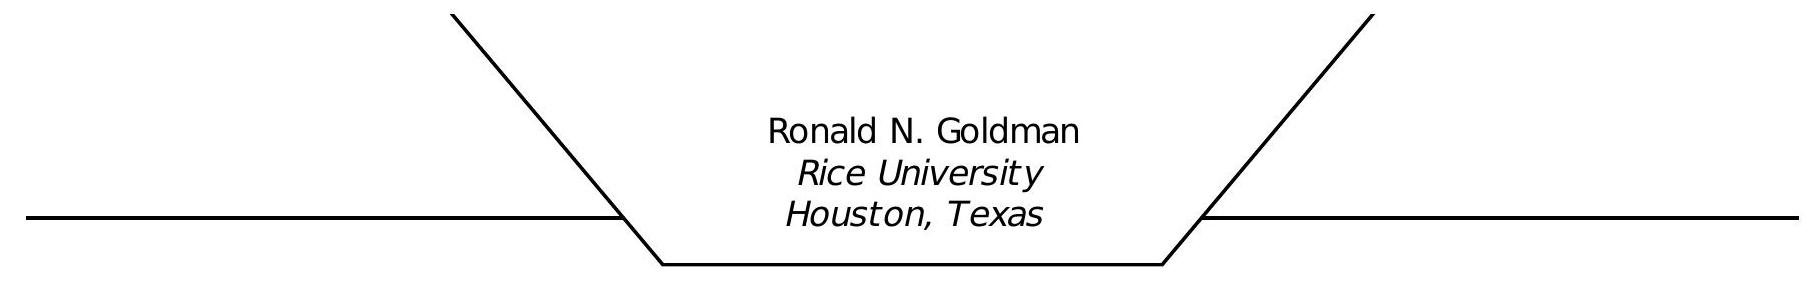
\includegraphics[max width=\textwidth]{2022_11_30_0cbb01a33d99487fc27fg-140}
\end{center}

Goal

Every nonsingular linear transformation of three-dimensional space is the product of three scales, two shears, and one rotation. The goal of this Gem is to show how to decompose any arbitrary, singular or nonsingular, linear or affine transformation of three-dimensional space into simple, geometrically meaningful, factors. For an alternative approach to similar problems (see Thomas, 1991).

\section{Nonsingular Linear Transformations}
Linear transformations of three-dimensional space are generally represented by $3 \times 3$ matrices. To decompose an arbitrary nonsingular linear transformation, consider, then, an arbitrary nonsingular $3 \times 3$ matrix L. We shall show that L can be factored into the product of three scales, two shears, and one rotation matrix.

Let the rows of L be given by the vectors $u, v$, w. Since the matrix L is nonsingular, the vectors $\mathrm{u}, \mathrm{v}, \mathrm{w}$ are linearly independent. Therefore, using the Gram-Schmidt orthogonalization procedure, we can generate 3 orthonormal vectors $u^{*}, v^{*}, w^{*}$ by setting

$$
\begin{aligned}
&\mathrm{u}^{*}=\mathrm{u} /|\mathrm{u}|, \\
&\mathrm{v}^{*}=\left(\mathrm{v}-\left(\mathrm{v} \cdot \mathrm{u}^{*}\right) \mathrm{u}^{*}\right) /\left|\mathrm{v}-\left(\mathrm{v} \cdot \mathrm{u}^{*}\right) \mathrm{u}^{*}\right|, \\
&\mathrm{w}^{*}=\left(\mathrm{w}-\left(\mathrm{w} \cdot \mathrm{u}^{*}\right) \mathrm{u}^{*}-\left(\mathrm{w} \cdot \mathrm{v}^{*}\right) \mathrm{v}^{*}\right) /\left|\mathrm{w}-\left(\mathrm{w} \cdot \mathrm{u}^{*}\right) \mathrm{u}^{*}-\left(\mathrm{w} \cdot \mathrm{v}^{*}\right) \mathrm{v}^{*}\right| .
\end{aligned}
$$

GRAPHICS GEMS III Edited by DAVID KIRK This orthogonalization procedure can be used to decompose the matrix L into the desired factors.

Begin with the rotation. By construction, the matrix $R$ whose rows are $u^{*}, v^{*}, w^{*}$ is an orthogonal matrix. If $\operatorname{Det}(R)=-1$, replace $w^{*}$ by $-w^{*}$. Then $R$ is the rotation matrix we seek. Using the results in Goldman (1991a), we can, if we like, retrieve the rotation axis and angle from the matrix R.

The three scaling transformations are also easy to find. Let

$$
\begin{aligned}
&\mathrm{s}_{1}=|\mathrm{u}|, \\
&\mathrm{s}_{2}=\left|\mathrm{v}-\left(\mathrm{v} \cdot \mathrm{u}^{*}\right) \mathrm{u}^{*}\right|, \\
&\mathrm{s}_{3}=\left|\mathrm{w}-\left(\mathrm{w} \cdot \mathrm{u}^{*}\right) \mathrm{u}^{*}-\left(\mathrm{w} \cdot \mathrm{v}^{*}\right) \mathrm{v}^{*}\right| .
\end{aligned}
$$

That is, $s_{1}, s_{2}, s_{3}$ are the lengths of $u^{*}, v^{*}, w^{*}$ before they are normalized. Now let $\mathrm{S}$ be the matrix with $\mathrm{s}_{1}, \mathrm{~s}_{2}, \mathrm{~s}_{3}$ along the diagonal and with zeroes everywhere else. The matrix $\mathrm{S}$ represents the three independent scaling transformations that scale by $s_{1}$ along the $x$-axis, $s_{2}$ along the $y$-axis, and $s_{3}$ along the z-axis. (If $\operatorname{Det}(R)$ was originally $-1$, then replace $s_{3}$ by $-s_{3}$. In effect, this mirrors points in the xy-plane.)

Before we can introduce the two shears, we need to recall notation for the identity matrix and the tensor product of two vectors.

Identity:

$$
I=\left|\begin{array}{lll}
1 & 0 & 0 \\
0 & 1 & 0 \\
0 & 0 & 1
\end{array}\right|
$$

\section{Tensor Product:}
$$
\nu \otimes \omega=\left|\begin{array}{lll}
v_{1} \omega_{1} & v_{1} \omega_{2} & v_{1} \omega_{3} \\
v_{2} \omega_{1} & v_{2} \omega_{2} & v_{2} \omega_{3} \\
v_{3} \omega_{1} & v_{3} \omega_{2} & v_{3} \omega_{3}
\end{array}\right|=\left|\begin{array}{l}
v_{1} \\
v_{2} \\
v_{3}
\end{array}\right| *\left|\omega_{1} \omega_{2} \omega_{3}\right|=v^{\mathrm{t}} * \omega .
$$

Here $*$ denotes matrix multiplication and the superscript $\mathrm{t}$ denotes

\section{III.3 DECOMPOSING LINEAR AND AFFINE TRANSFORMATIONS}
transpose. Observe that for all vectors $\mu$

$$
\begin{gathered}
\mu \cdot \mathrm{I}=\mu, \\
\mu *(\nu \otimes \omega)=(\mu \cdot v) \omega .
\end{gathered}
$$

Now we are ready to define the two shears. Recall from Goldman (199lb) that a shear $\mathrm{H}$ is defined in terms of a unit vector $\mathrm{v}$ normal to a plane $Q$, a unit vector $\omega$ in the plane $Q$, and an angle $\varphi$ by setting

$$
\mathrm{H}=\mathrm{I}+\tan \varphi(v \otimes \omega) .
$$

Let $\mathrm{H}_{1}$ be the shear defined by unit normal $v^{*}$, the unit vector $\mathrm{u}^{*}$, and the angle $\theta$ by setting

$$
\begin{aligned}
&\mathrm{H}_{1}=\mathrm{I}+\tan \theta\left(\mathrm{v}^{*} \otimes \omega^{*}\right), \\
&\tan \theta=\mathrm{v} \cdot \mathrm{u}^{*} / \mathrm{s}_{2} .
\end{aligned}
$$

Similarly, let $\mathrm{H}_{2}$ be the shear defined by unit normal $\mathrm{w}^{*}$, the unit vector $r^{*}$, and the angle $\psi$ by setting

$$
\begin{gathered}
\mathrm{H}_{2}=\mathrm{I}+\tan \psi\left(\mathrm{w}^{*} \otimes \mathrm{r}^{*}\right), \\
\tan \psi=\operatorname{SQRT}\left\{\left(\mathrm{w} \cdot \mathrm{u}^{*}\right)^{2}+\left(\mathrm{w} \cdot \mathrm{v}^{*}\right)^{2}\right\} / \mathrm{s}_{3^{\prime}} \\
\mathrm{r}^{*}=\left\{\left(\mathrm{w} \cdot \mathrm{u}^{*}\right) \mathrm{u}^{*}+\left(\mathrm{w} \cdot \mathrm{v}^{*}\right) \mathrm{v}^{*}\right\} \mathrm{s}_{3} \tan \psi
\end{gathered}
$$

Then it is easy to verify that

$$
\begin{aligned}
&\mathrm{u}^{*} * \mathrm{H}_{1}=\mathrm{u}^{*}, \quad \mathrm{v}^{*} * \mathrm{H}_{1}=\mathrm{v}^{*}+\left(\mathrm{v} \cdot \mathrm{u}^{*} / \mathrm{s}_{2}\right) \mathrm{u}^{*}, \quad \mathrm{w}^{*} * \mathrm{H}_{1}=\mathrm{w}^{*}, \\
&\mathrm{u}^{*} * \mathrm{H}_{2}=\mathrm{u}^{*}, \quad \mathrm{v}^{*} * \mathrm{H}_{2}=\mathrm{v}^{*}, \\
&\mathrm{w}^{*} * \mathrm{H}_{2}=\mathrm{w}^{*}+\left\{\left(\mathrm{w} \cdot \mathrm{u}^{*}\right) \mathrm{u}^{*}+\left(\mathrm{w} \cdot \mathrm{v}^{*}\right) \mathrm{v}^{*}\right\} / \mathrm{s}_{3} .
\end{aligned}
$$

Finally, we shall show that

$$
\mathrm{L}=\mathrm{S} * \mathrm{R} * \mathrm{H}_{1} * \mathrm{H}_{2}
$$

Since the transformation L is linear, we need only check that both sides give the same result on the canonical basis $\mathbf{i}, \mathbf{j}, \mathbf{k}$. By construction we know that

$$
\mathbf{i} * \mathrm{~L}=\mathrm{u}, \quad \mathbf{j} * \mathrm{~L}=\mathrm{v}, \quad \mathbf{k} * \mathrm{~L}=\mathrm{w},
$$

so we need to verify that we get the same results for the right-hand side. Let us check.

First,

$$
\begin{aligned}
\mathbf{i} * \mathrm{~S} * \mathrm{R} * \mathrm{H}_{1} * \mathrm{H}_{2} &=\left(\mathrm{s}_{1}\right) \mathbf{i} * \mathrm{R} * \mathrm{H}_{1} * \mathrm{H}_{2} \\
&=\left(\mathrm{s}_{1}\right) \mathrm{u}^{*} * \mathrm{H}_{1} * \mathrm{H}_{2} \\
&=\mathrm{u} .
\end{aligned}
$$

since by construction the two shears $\mathrm{H}_{1}$ and $\mathrm{H}_{2}$ do not affect $\mathrm{u}^{*}$. Next,

$$
\begin{aligned}
\mathbf{j} * \mathrm{~S} * \mathrm{R} * \mathrm{H}_{1} * \mathrm{H}_{2} &=\left(\mathrm{s}_{2}\right) \mathbf{j} * \mathrm{R} * \mathrm{H}_{1} * \mathrm{H}_{2} \\
&=\left(\mathrm{s}_{2}\right) \mathrm{v}^{*} * \mathrm{H}_{1} * \mathrm{H}_{2} \\
&=\left\{\mathrm{s}_{2} \mathrm{v}^{*}+\left(\mathrm{v} \cdot \mathrm{u}^{*}\right) \mathrm{u}^{*}\right\} * \mathrm{H}_{2} \\
&=\mathrm{s}_{2} \mathrm{v}^{*}+\left(\mathrm{v} \cdot \mathrm{u}^{*}\right) \mathrm{u}^{*} \\
&=\mathrm{v} .
\end{aligned}
$$

Finally,

$$
\begin{aligned}
\mathbf{k} * \mathrm{~S} * \mathrm{R} * \mathrm{H}_{1} * \mathrm{H}_{2} &=\left(\mathrm{s}_{3}\right) \mathbf{k} * \mathrm{R} * \mathrm{H}_{1} * \mathrm{H}_{2} \\
&=\left(\mathrm{s}_{3}\right) \mathrm{w}^{*} * \mathrm{H}_{1} * \mathrm{H}_{2} \\
&=\left(\mathrm{s}_{3}\right) \mathrm{w}^{*} * \mathrm{H}_{2} \\
&=\mathrm{s}_{3} \mathrm{w}^{*}+\left(\mathrm{w} \cdot \mathrm{u}^{*}\right) \mathrm{u}^{*}+\left(\mathrm{w} \cdot \mathrm{v}^{*}\right) \mathrm{v}^{*} \\
&=\mathrm{w} .
\end{aligned}
$$

\section{III.3 DECOMPOSING LINEAR AND AFFINE TRANSFORMATIONS}
Although we have succeeded in factoring an arbitrary nonsingular linear transformation, notice that this decomposition is not unique. Indeed, the Gram-Schmidt orthogonalization procedure depends upon the ordering of the vectors to which it is applied. We could, for example, have applied the Gram-Schmidt procedure to the vectors in the order w, u, v instead of $u, v$, w. We would then have retrieved a different decomposition of the same matrix. Nevertheless, this procedure is still of some value since it allows us to decompose an arbitrary nonsingular linear transformation into simple, geometrically meaningful factors.

\section{Singular Linear Transformations}
Now let L be an arbitrary singular $3 \times 3$ matrix. There are three cases to consider, depending on the rank of L. If $\operatorname{rank}(\mathrm{L})=0$, there is nothing to do since L simply maps all vectors into the zero vector. The case $\operatorname{rank}(\mathrm{L})=1$ is also essentially trivial, since all vectors are simply appropriately scaled and then projected onto a single fixed vector. Therefore, we shall concentrate on the case where $\operatorname{rank}(\mathrm{L})=2$.

We will show that when $\operatorname{rank}(\mathrm{L})=2$, we still need one rotation, but we require only two scales, one shear, and one parallel projection. Thus, the number of scales is reduced by one and a shear is replaced by a parallel projection. Moreover, we shall shovv that the parallel projection can be replaced by a shear followed by an orthogonal projection.

Again, let the rows of L be given by the vectors $u, v$, w. Since the matrix $L$ is singular, the row vectors $u, v, w$ are linearly dependent, but since $\operatorname{rank}(\mathrm{L})=2$, two rows of $\mathrm{L}$ are linearly independent. For simplicity and without loss of generality, we will assume that $u$ and $v$ are linearly independent.

Modifying the Gram-Schmidt orthogonalization procedure, we can generate three orthonormal vectors $u^{*}, v^{*}, w^{*}$ by setting

$$
\begin{aligned}
u^{*} &=u /|u|, \\
v^{*} &=\left(v-\left(v \cdot u^{*}\right) u^{*}\right) /\left|v-\left(v \cdot u^{*}\right) u^{*}\right|, \\
w^{*} &=u^{*} \times v^{*} .
\end{aligned}
$$

This orthogonalization procedure can again be used to decompose the matrix L into the desired factors.

By construction, the matrix $R$ whose rows are $u^{*}, v^{*}, w^{*}$ is an orthogonal matrix and $\operatorname{Det}(\mathrm{R})=1$. The matrix $\mathrm{R}$ is the rotation matrix that we seek. We can recover the axis and angle of rotation from the matrix $\mathrm{R}$ using the techniques described in Goldman (199la).

The two scaling transformations are also easy to find. Let

$$
\begin{aligned}
&\mathrm{s}_{1}=|\mathrm{u}|, \\
&\mathrm{s}_{2}=\left|\mathrm{v}-\left(\mathrm{v} \cdot \mathrm{u}^{*}\right) \mathrm{u}^{*}\right| .
\end{aligned}
$$

Note that $s_{1}, s_{2}$ are, respectively, the lengths of $u^{*}, v^{*}$ before they are normalized. Now let $\mathrm{S}$ be the matrix with $\mathrm{s}_{1}, \mathrm{~s}_{2}, 1$ along the diagonal and with zeroes everywhere else. The matrix $S$ represents the two independent scaling transformations that scale by $\mathrm{s}_{1}$ along the $\mathrm{x}$-axis and $\mathrm{s}_{2}$ along the y-axis.

The shear $\mathrm{H}$ is the same as the first of the two shears that we used to decompose a nonsingular linear transformation. Using the notation for the identity matrix and the tensor product of two vectors that we established above,

$$
\begin{aligned}
\mathrm{H} &=\mathrm{I}+\tan \theta\left(\mathrm{v}^{*} \otimes \mathrm{u}^{*}\right), \\
\tan \theta &=\mathrm{v} \cdot \mathrm{u}^{*} / \mathrm{s}_{2} .
\end{aligned}
$$

Thus, $\mathrm{H}$ is the shear defined by the unit normal vector $\mathrm{v}^{*}$, the unit vector $u^{*}$, and the angle $\theta$. Again, it is easy to verify that

$$
u^{*} * H=u^{*}, \quad v^{*} * H=v^{*}+\left(v \cdot u^{*} / s_{2}\right) u^{*}, \quad w^{*} * H=w^{*} .
$$

Last, we define the parallel projection $P$ to be projection into the $u^{*} v^{*}$-plane parallel to the vector( $\left.w^{*}-\mathrm{w}\right)$. According to Goldman(1990), the matrix $\mathrm{P}$ is given by

$$
\mathrm{P}=\mathrm{I}-\mathrm{w}^{*} \otimes\left(\mathrm{w}^{*}-\mathrm{w}\right)
$$

Notice that if $\mathrm{w}=0$, this parallel projection reduces to orthogonal projection into the $u^{*} v^{*}$-plane (Goldman, 1990). In any event, it is easy

\section{III.3 DECOMPOSING LINEAR AND AFFINE TRANSFORMATIONS}
to verify that

$$
\mathrm{u}^{*} * \mathrm{P}=\mathrm{u}^{*}, \quad \mathrm{v}^{*} * \mathrm{P}=\mathrm{v}^{*}, \quad \mathrm{w}^{*} * \mathrm{P}=\mathrm{w} .
$$

Finally, let us show that

$$
\mathrm{L}=\mathrm{S} * \mathrm{R} * \mathrm{H} * \mathrm{P}
$$

by checking that both sides give the same result on the canonical basis $\mathbf{i}, \mathbf{j}$, k. By construction we know that

$$
\mathbf{i} * \mathrm{~L}=\mathrm{u}, \quad \mathbf{j} * \mathrm{~L}=\mathrm{v}, \quad \mathbf{k} * \mathrm{~L}=\mathrm{w},
$$

so we need to verify that we get the same results for the right-hand side. Let us check.

First,

$$
\begin{aligned}
\mathbf{i} * \mathrm{~S} * \mathrm{R} * \mathrm{H} * \mathrm{P} &=\left(\mathrm{s}_{1}\right) \mathbf{i} * \mathrm{R} * \mathrm{H} * \mathrm{P} \\
&=\left(\mathrm{s}_{1}\right) \mathrm{u}^{*} * \mathrm{H} * \mathrm{P} \\
&=\mathrm{s}_{1} \mathrm{u}^{*} \\
&=\mathrm{u},
\end{aligned}
$$

since by construction the two linear transformations $\mathrm{H}$ and $\mathrm{P}$ do not affect $u^{*}$.

Next,

$$
\begin{aligned}
\mathbf{j} * \mathrm{~S} * \mathrm{R} * \mathrm{H} * \mathrm{P} &=\left(\mathrm{s}_{2}\right) \mathbf{j} * \mathrm{R} * \mathrm{H} * \mathrm{P} \\
&=\left(\mathrm{s}_{2}\right) \mathrm{v}^{*} * \mathrm{H} * \mathrm{P} \\
&=\left\{\mathrm{s}_{2} \mathrm{v}^{*}+\left(\mathrm{v} \cdot \mathrm{u}^{*}\right) \mathrm{u}^{*}\right\} * \mathrm{P} \\
&=\mathrm{s}_{2} \mathrm{v}^{*}+\left(\mathrm{v} \cdot \mathrm{u}^{*}\right) \mathrm{u}^{*} \\
&=\mathrm{v} .
\end{aligned}
$$

\section{III.3 DECOMPOSING LINEAR AND AFFINE TRANSFORMATIONS}
Finally,

$$
\begin{aligned}
\mathbf{k} * \mathrm{~S} * \mathrm{R} * \mathrm{H} * \mathrm{P} &=\mathbf{k} * \mathrm{R} * \mathrm{H} * \mathrm{P} \\
&=\mathrm{w}^{*} * \mathrm{H} * \mathrm{P} \\
&=\mathrm{w}^{*} * \mathrm{P} \\
&=\mathrm{w} .
\end{aligned}
$$

By the way, every parallel projection can be written as the product of a shear followed by an orthogonal projection. To see this, recall that a projection $P$ parallel to the vector $\omega$ into the plane with normal vector $n$ is given by Goldman (1990):

$$
P=I-(n \otimes \omega) / n \cdot \omega .
$$

Consider the orthogonal projection 0 into the plane perpendicular to the unit vector $n$ (Goldman, 1990),

$$
0=I-(n \otimes n),
$$

and the shear $\mathrm{K}$ defined by the unit normal vector $\mathrm{n}$, the unit vector $v=(\mathrm{n}-\omega / \omega \cdot \mathrm{n}) /|\mathrm{n}-\omega / \omega \cdot \mathrm{n}|$, and the angle $\theta$ given by $\tan \theta=$ $|\mathrm{n}-\omega / \omega \cdot \mathrm{n}|:$

$$
K=I+\tan \theta(n \otimes \nu) .
$$

Since $v \cdot \mathrm{n}=0$, it follows that $(\mathrm{n} \otimes v) *(\mathrm{n} \otimes \mathrm{n})=(v \cdot \mathrm{n})(\mathrm{n} \otimes \mathrm{n})=0$. Therefore,

$$
I-(n \otimes \omega) / n \cdot \omega=\{1+\tan \theta(n \otimes \nu)\} *\{I-(n \otimes n)\},
$$

or, equivalently,

$$
\mathrm{P}=\mathrm{K} * 0
$$

In our case $\omega=\mathrm{w}^{*}-\mathrm{w}, \mathrm{n}=\mathrm{w}^{*}$, and $v=\mathrm{w}$. Thus, we have shown that when $\operatorname{rank}(\mathrm{L})=2$, we can factor L into the product of two scales one rotation, two shears, and one orthogonal projection. This decomposition is the same as in the nonsingular case, except that the number of scales is reduced by one and the standard nonsingular factors-scales, rotation, and shears-are followed by an orthogonal projection.

\section{III.3 DECOMPOSING LINEAR AND AFFINE TRANSFORMATIONS}
Notice again that this decomposition is not unique. Indeed, the modified Gram-Schmidt orthogonalization procedure also depends upon the ordering of the vectors to which it is applied. We could, for example, have applied the Gram-Schmidt procedures to the vectors in the order $v$, u instead of $u$, v. We would then have retrieved a different decomposition of the same matrix. Nevertheless, this procedure is still of some value since it allows us to decompose an arbitrary singular linear transformation into simple, geometrically meaningful factors.

\section{Affine Transformations}
Finally, recall that every affine transformation A is simply a linear transformation $\mathrm{L}$ followed by a translation $\mathrm{T}$. If the affine transformation is represented by a $4 \times 3$ matrix

$$
\mathrm{A}=\left|\begin{array}{l}
\mathrm{L} \\
\mathrm{T}
\end{array}\right|,
$$

then the upper $3 \times 3$ submatrix L represents the linear transformation and the fourth row $\mathrm{T}$ represents the translation vector. Thus, to decompose an arbitrary affine transformation into simpler, geometrically meaningful factors, simply factor the associated linear transformation L and append the translation T. Thus, every nonsingular affine transformation of three-dimensional space can be factored into the product of three scales, two shears, one rotation, and one translation. Similarly, every singular affine transformation of three-dimensional space can be factored into the product of two scales, two shears, one rotation, one orthogonal projection, and one translation. Again, these decompositions are not unique, since the decompositions of the associated linear transformations are not unique. Nevertheless, these procedures are still of some value since they allow us to decompose arbitrary affine transformations into simple, geometrically meaningful factors.

See also G2, 319; G2, 320; G3, C.2.\\
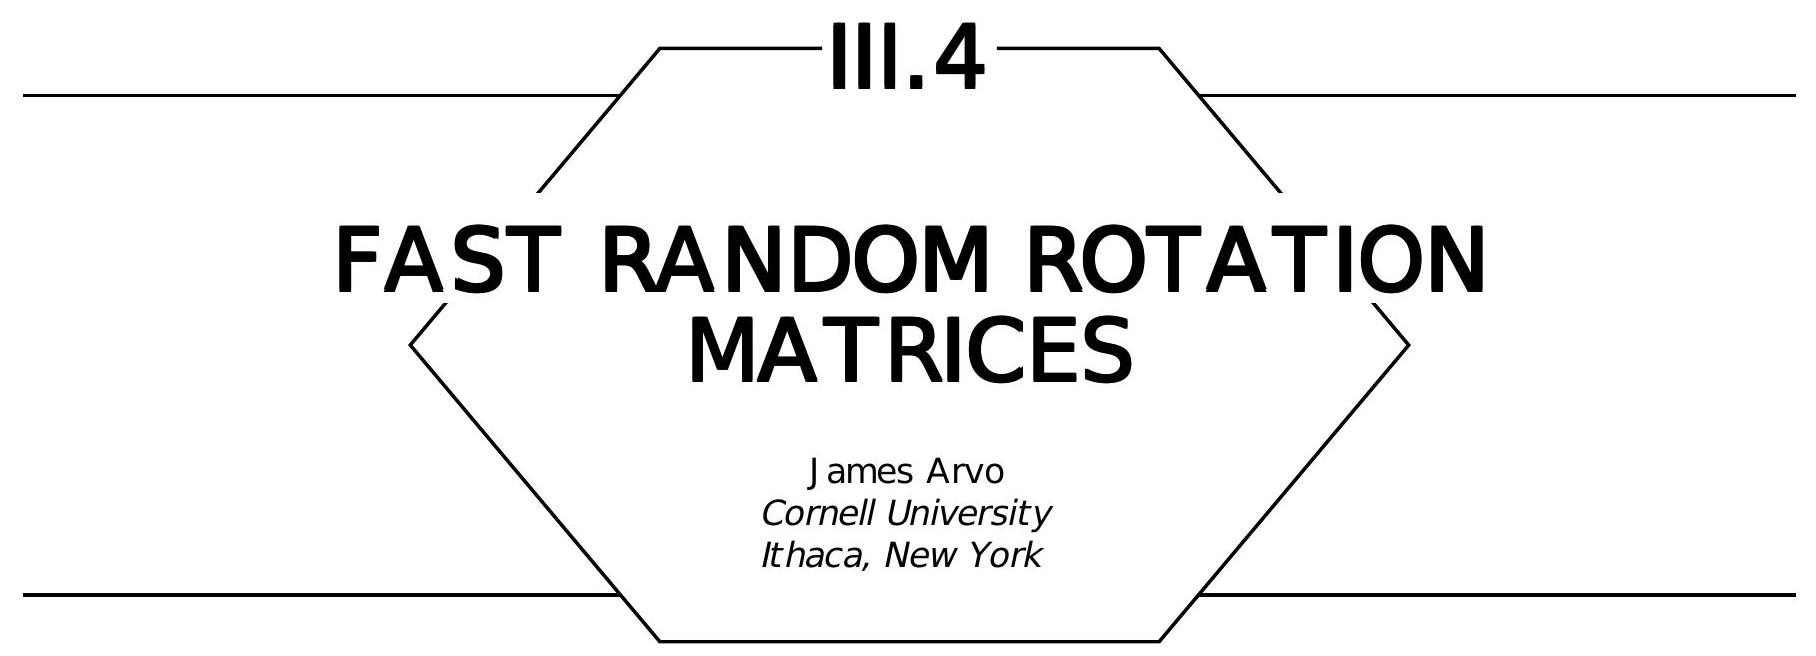
\includegraphics[max width=\textwidth, center]{2022_11_30_0cbb01a33d99487fc27fg-149}

In a previous Gem (Arvo, 1991), I described a method for generating random rotation matrices based on random unit quaternions. As Ken Shoemake points out in his Gem (III.6) that algorithm was flawed in that it did not generate uniformly distributed rotation matrices. For a method based on quaternions that corrects this defect see his algorithm. In this Gem I describe a completely different approach to solving the same problem that has the additional benefit of being slightly faster than the previous method. The approach is based on the following fact:

To generate uniformly distributed random rotations of a unit sphere, first perform a random rotation about the vertical axis, then rotate the north pole to a random position.

The first step of this prescription is trivial. Given a random number, $\mathrm{x}_{1}$, between 0 and 1. the matrix $\mathrm{R}$ does the trick:

$$
R=\begin{array}{ccc}
\cos \left(2 \pi \mathrm{x}_{1}\right) & \sin \left(2 \pi \mathrm{x}_{1}\right) & 0 \\
-\sin \left(2 \pi \mathrm{x}_{1}\right) & \cos \left(2 \pi \mathrm{x}_{1}\right) & 0 \\
0 & 0 & 1
\end{array} .
$$

Here we are assuming that the z-axis is the vertical axis, so the "north pole" will be the point $\mathrm{z}=(0,0,1)$. The second operation is not quite so obvious, but fortunately it can be carried out quite efficiently. Observe that we can take the point $\mathrm{z}$ to any other point $\mathrm{p}$ on the sphere via a

\section{III.4 FAST RANDOM ROTATION MATRICES}
reflection through the plane orthogonal to the line $\overline{\mathrm{zp}}$ and containing the origin. Such a reflection is given by the Householder matrix

$$
H=I-2 v^{T},
$$

where $\mathrm{v}$ is a unit vector parallel to $\overline{\mathrm{zp}}$ (see, for instance, Golub and Van Loan, 1985). To turn this into a rotation we need only apply one more reflection (making the determinant positive). A convenient reflection for this purpose is reflection through the origin-that is, scaling by $-1$. Thus, the final rotation matrix can be expressed as the product

$$
M=-H R,
$$

where $R$ is the simple rotation in Eq. (1). The rotation matrix M will be uniformly distributed within $\mathrm{SO}(3)$, the set of all rotations in three-space, if $\mathrm{H}$ takes the north pole to every point on the sphere with equal probability density. This will hold if the image of z under the random reflection is such that both its azimuth angle and the cosine of its elevation angle are uniformly distributed. The matrix $\mathrm{H}$ in Eq. (2) will satisfy these requirements if we let

$$
\mathrm{v}=\begin{gathered}
\cos \left(2 \pi \mathrm{x}_{2}\right) \sqrt{\mathrm{x}_{3}} \\
\sin \left(2 \pi \mathrm{x}_{2}\right) \sqrt{\mathrm{x}_{3}} \\
\sqrt{1-\mathrm{x}_{3}}
\end{gathered},
$$

where $x_{2}$ and $x_{3}$ are two independent uniform random variables in $[0,1]$. To show this we need only compute $p=H z$ and verify that $p$ is distributed appropriately. Using the preceding definition of $\mathrm{v}$, we have

$$
p=z-2 v^{T} z=\begin{gathered}
-2 \cos \left(2 \pi x_{2}\right) \sqrt{x_{3}\left(1-\mathrm{x}_{3}\right)} \\
-2 \sin \left(2 \pi x_{2}\right) \sqrt{x_{3}\left(1-\mathrm{x}_{3}\right)} \\
2 \mathrm{x}_{3}-1
\end{gathered} .
$$

Because the third component of $p$ is the cosine of its elevation angle, we see immediately that it is uniformly distributed over $[-1,1]$, as required.

\section{III.4 FAST RANDOM ROTATION MATRICES}
random\_rotation $\left(x_{1}, x_{2}, x_{2}, M\right)$

$x_{1}, x_{2}, x_{3}$ : real; Three random variables.

$M$ : matrix3; The resulting matrix.

begin

$\theta \leftarrow 2 \pi x_{1} ; \quad$ Pick a rotation about the pole.

$\phi \leftarrow 2 \pi x_{2} ; \quad$ Pick a direction to deflect the pole.

$z \leftarrow x_{3} ; \quad$ Pick the amount of pole deflection.

Construct a vector for performing the reflection.

$V \leftarrow\left[\begin{array}{c}\cos \phi \sqrt{z} \\ \sin \phi \sqrt{z} \\ \sqrt{1-z}\end{array}\right]$

Construct the rotation matrix by combining two

simple rotations: first rotate about the $Z$ axis,

then rotate the $Z$ axis to a random orientation.

$M \leftarrow\left(2 V V^{\mathrm{T}}-I\right)\left[\begin{array}{ccc}\cos \theta & \sin \theta & 0 \\ -\sin \theta & \cos \theta & 0 \\ 0 & 0 & 1\end{array}\right]$

end

Figure 1. An efficient procedure for creating random $3 \times 3$ rotation matrices.

Similarly, from its first two components we see that the azimuth angle of $p$ is $2 \pi x_{2}$, which is uniformly distributed over $[0,2 \pi]$.

The complete algorithm combining the reflection and simple rotation is shown in Fig. 1, and an optimized version in C appears in the appendix. Procedure "random\_rotation" requires three uniformly distributed random numbers between 0 and 1. Supplying these values as arguments has several advantages. First, the procedure can be used in conjunction with your favorite pseudorandom number generator, and there are a great many to choose from. Secondly, if we obtain the three random numbers by stratified or jittered sampling of the unit cube, the resulting rotation

\section{III.4 FAST RANDOM ROTATION MATRICES}
\begin{center}
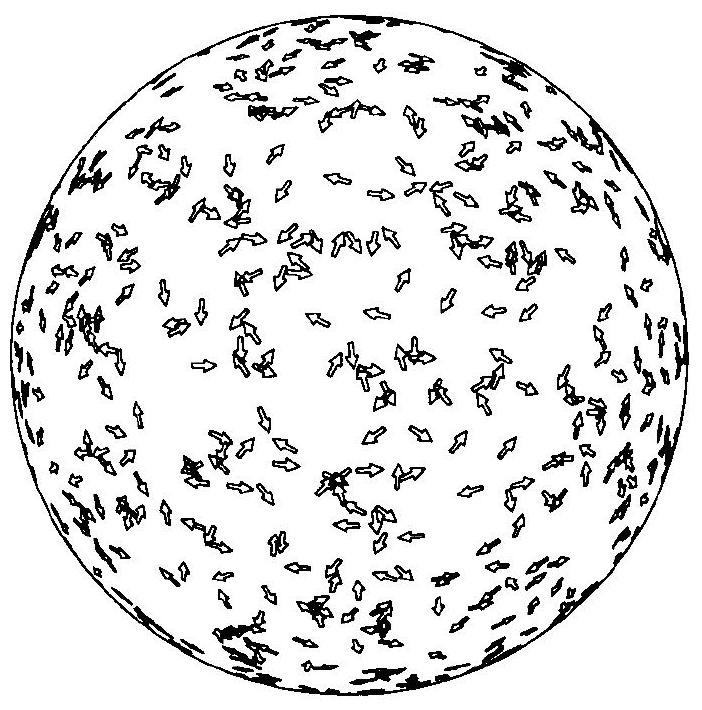
\includegraphics[max width=\textwidth]{2022_11_30_0cbb01a33d99487fc27fg-152}
\end{center}

(a)

\begin{center}
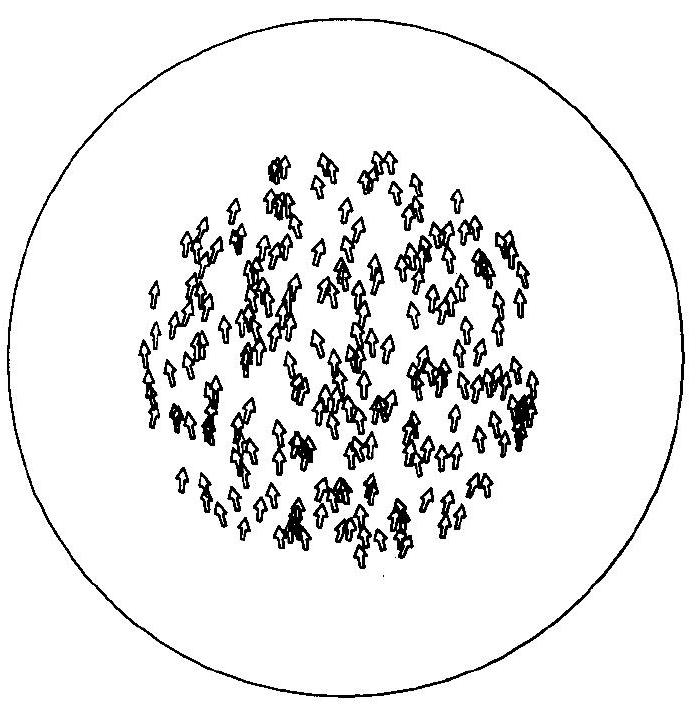
\includegraphics[max width=\textwidth]{2022_11_30_0cbb01a33d99487fc27fg-152(1)}
\end{center}

(b)

Figure 2.

matrices will inherit the benefits-namely, less clumping. Finally, if we restrict the range of the random input variables (while maintaining their uniformity), we can generate uniformly distributed perturbations or "wobbles" within given limits.

Figure $2 \mathrm{a}$ shows the result of applying 1,000 random rotations to a sphere with an arrow painted at one pole. The resulting pattern looks much the same from any vantage point, providing visual confirmation of uniformity. Figure $2 \mathrm{~b}$ was generated by restricting $\mathrm{x}_{1}$ and $\mathrm{x}_{3}$ to the range $[0,0.1]$

See also G2, 355; G3, C.6.

\begin{center}

\includegraphics[max width=\textwidth]{2022_11_30_0cbb01a33d99487fc27fg-153}
\end{center}

\section{Introduction}
Spencer, (1991) explains how to express a matrix as a set of parameters, called an unmatrix. In Spencer's unmatrix, each parameter is a single value that can be interpolated using linear interpolation or piecewise splining techniques. When simple interpolation is used to calculate transformations between samples, unnatural motion can occur.

This Gem shows how to interpolate motion naturally between two sample matrices for use in motion control or key-framing applications. This technique was used to create the key frame animation system described in Dana (1991).

\section{Interpolating in Logarithmic Space}
Unnatural or accelerated motion occurs when scaling parameters are interpolated in a straightforward way. A simple interpolation, halfway between a scaling parameter of $0.50$ and 2.0, produces a value of $1.25$ when the visually expected value would be 1.0.

A solution to this problem is to interpolate the logarithm of the scaling parameter.

\section{III.5 ISSUES AND TECHNIQUES FOR KEYFRAMING TRANSFORMATIONS}
\section{Relative Motion}
The most natural motion from one sample transformation to another is the one that takes the shortest apparent path. When rotation parameters are interpolated, sometimes the shortest path may cross the zero degree mark. For example, the shortest path between 10 degrees and 350 degrees is $-20$ degrees, not $+340$ degrees.

A second rotation problem occurs when you want an object to appear to rotate relative to its own oriental ion instead of relative to its current orientation in the 3-D universe.

To get the desired transformation and to solve both the zero mark problem and the axis problem:

\begin{enumerate}
  \item Express the motion between two samples relative to the first sample, prior to interpolation.

  \item Calculate the interpolation using an identity transformation and the difference between the two samples.

  \item Concatenate the interpolated transformation to the first sample.

\end{enumerate}

This solves the zero mark problem because the rotational values of an identity transformation are all zero. It also solves the axis problem by expressing a segment of motion relative to the segment's first sample.

\section{Linear vs. Splined Interpolation}
Although it might seem best to use a splining technique to interpolate all the parameters of an unmatrix, experience has shown that ordinary linear interpolation is best for the scaling, shearing, rotation, and perspective parameters, and splined interpolation is best for the translation parameters.

\section{III.5 ISSUES AND TECHNIQUES FOR KEYFRAMING TRANSFORMATIONS}
\section{Subdividing Motion}
For a motion to have constant speed between two samples, the motion must be subdivided into intervals of equal length in space, not just duration in time. When using splined interpolation to interpolate translation parameters, the spline type must allow for even subdivision along the length of a piece. A spline, such as a Cardinal spline, should be used.

See also G3, C.7.\\

\includegraphics[max width=\textwidth, center]{2022_11_30_0cbb01a33d99487fc27fg-156}

\section{Background}
A previous Graphics Gem (Arvo, 1991) presented an algorithm for generating random rotations, in both quaternion and matrix form. It takes as input three uniform deviates and efficiently computes a random rotation with a uniformly distributed axis and a uniformly distributed angle. The purpose of the present gem is to demonstrate that, surprisingly, that algorithm does not generate a uniformly distributed rotation, and to give two simple algorithms that do.

How can the distribution of the axis and angle be uniform, and yet the distribution of the rotations not be? To answer that question requires, first of all, a definition of uniformity. Since rotations form a group, an approach that is both standard and intuitively satisfying uses "Haar measure" as follows: If $\mathrm{X}$ is a random rotation with uniform distribution, then for any fixed but arbitrary rotation R, RX and XR have the same distribution as $X$. A rough physical analogy is the testing of a bicycle wheel for balance by spinning it and looking for wobbles, or dragging a flat edge across freshly poured cement to smooth it.

\section{Planar Rotations}
Before examining the implications of this definition for spatial rotations, let us first examine its application to the simpler case of planar rotations, where we can use both our eyes and our intuition. A planar rotation can be represented in several ways, for example as an angle between 0 and

\section{III.6 UNIFORM RANDOM ROTATIONS}
$2 \pi$, as a unit complex number $\mathrm{x}+\mathbf{i} \mathrm{y}=\cos \theta+\mathbf{i} \sin \theta$, and as a matrix

\begin{center}
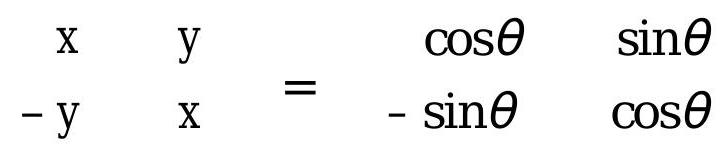
\includegraphics[max width=\textwidth]{2022_11_30_0cbb01a33d99487fc27fg-157}
\end{center}

Planar rotations combine by summing their angles modulo $2 \pi$, so one way to generate a uniform planar rotation is to generate a uniform angle. Combination of $\mathrm{X}$ with $\mathrm{R}$ merely slides the angle around. Since this leaves the distribution unchanged, it is uniform. A more geometrical interpretation of this problem is that we want to generate points uniformly distributed on the unit circle $x^{2}+y^{2}=1$, with probability proportional to arc length. Note that the average magnitude of $x$ will be $1 / \pi$ times the integral of $2 \cos \theta$ from 0 to $\pi / 2$, namely $2 / \pi \approx 0.6366$. This computation is merely "summing"-integrating-the $\mathrm{x}$ values of all the points on the right half of the circle and dividing by the "number of points" used-the arc length of that half of the circle. Here and subsequently we take advantage of circle (later, sphere) and sinusoid symmetries when computing magnitudes. Now suppose a rotation is generated by choosing a uniformly distributed $\mathrm{x}$ between $-1$ and $+1$, with $\mathrm{y}$

\begin{center}
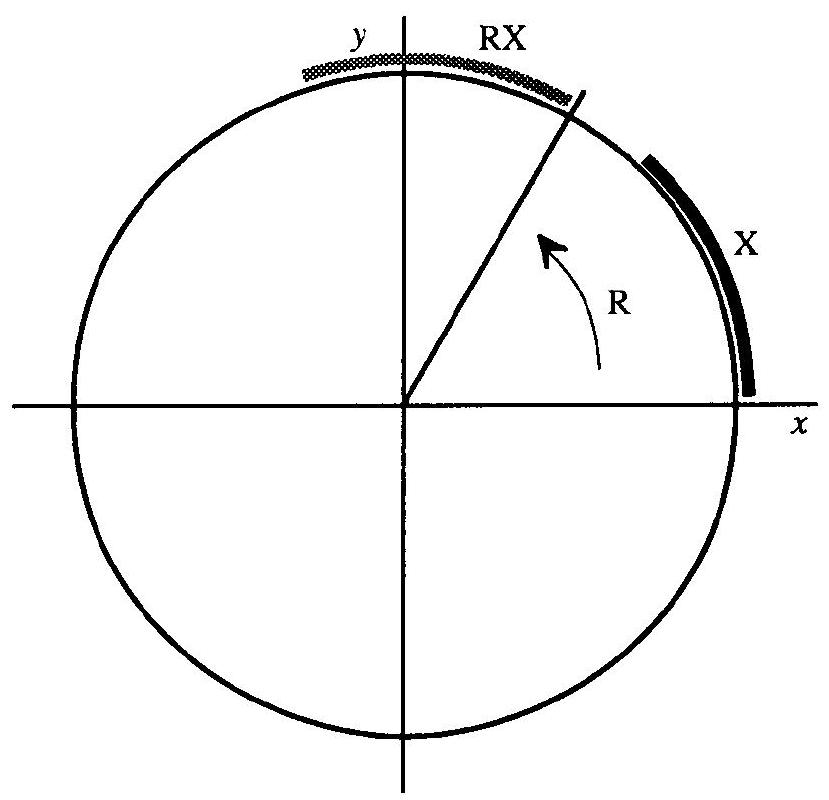
\includegraphics[max width=\textwidth]{2022_11_30_0cbb01a33d99487fc27fg-157(1)}
\end{center}

Figure 1. Haar test reveals distribution lumps.

\section{III.6 UNIFORM RANDOM ROTATIONS}
computed as $\pm \sqrt{1-x^{2}}$ (either sign being equally likely). For this distribution the average magnitude of $\mathrm{x}$ will be $\frac{1}{2}$, and so it cannot give uniformly distributed rotations.

\section{Uniform Spherical Distribution}
Shortly, we are going to want to know about points uniformly distributed on a sphere, and on a hypersphere. The sphere case is easier to visualize, and has a surprising result: Each coordinate of a point uniformly distributed on a sphere is uniformly distributed! Thus, for example, the average magnitude of the $x$ coordinate is $\frac{1}{2}$. A uniformly distributed point can be generated by choosing $z$ uniformly distributed on $-1$ to $+1$, and $\mathrm{x}$ and $\mathrm{y}$ uniformly distributed on a circle of radius $\sqrt{1-\mathrm{z}^{2}}$, a fact exploited in Arvo's algorithm (Arvo, 1991).

To derive the $\mathrm{x}$ distribution and average magnitude, we integrate circular slices. Since the sphere is symmetrical, and only positive $\mathrm{x}$ values lie in the right hemisphere, we will confine our attention there.

\begin{center}
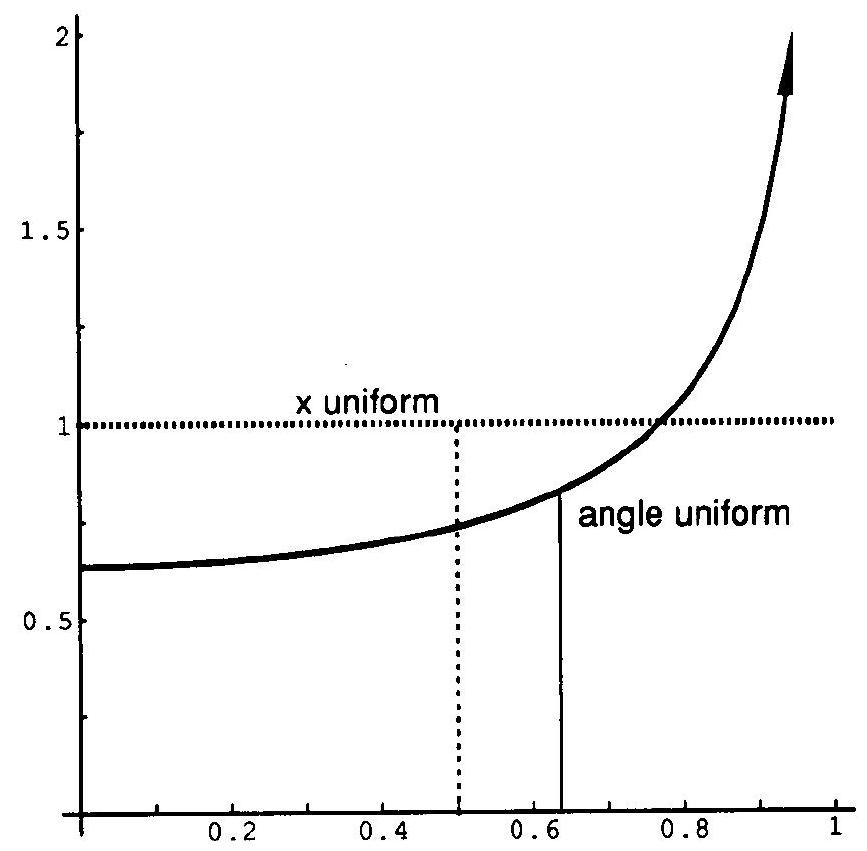
\includegraphics[max width=\textwidth]{2022_11_30_0cbb01a33d99487fc27fg-158}
\end{center}

Figure 2. Density and average of $\mathrm{x}$ for planar rotation.

\section{III.6 UNIFORM RANDOM ROTATIONS}
Calculation will be simpler if the variable of integration is $\theta$, with $\mathrm{x}=\sin \theta$; then the radius of the circular slice at $\mathrm{x}$ will be $\cos \theta$, and its perimeter length $2 \pi \cos \theta$. The area of the hemisphere is, of course, just the integral of the perimeters for $\theta$ from 0 to $\pi / 2$, which is $2 \pi$. For the circle, the integral for average magnitude weighted each $\mathrm{x}$ value by 2 , since the one-dimensional slices gave exactly two points. Now the weight for $\mathrm{x}=\sin \theta$ will be $2 \pi \cos \theta$, because of the circular slice. (There, $\mathrm{x}$ was $\cos \theta$; here, $\sin \theta$.) So the average magnitude is

$$
\frac{1}{2 \pi} \int^{\pi / 2}-2 \pi \cos \theta \sin \theta \mathrm{d} \theta=\frac{1}{2} .
$$

To find the probability of a value being between 0 and $\mathrm{x}$, we simply integrate the circular slices from 0 to arcsin $\mathrm{x}$, giving

$$
\frac{1}{2 \pi} \int_{0}^{\arcsin x}-2 \pi \cos \theta \mathrm{d} \theta=\mathrm{x} \text {. }
$$

This shows that the coordinate distributions are uniform (though not independently so!) for points uniformly distributed on a sphere.

\begin{center}
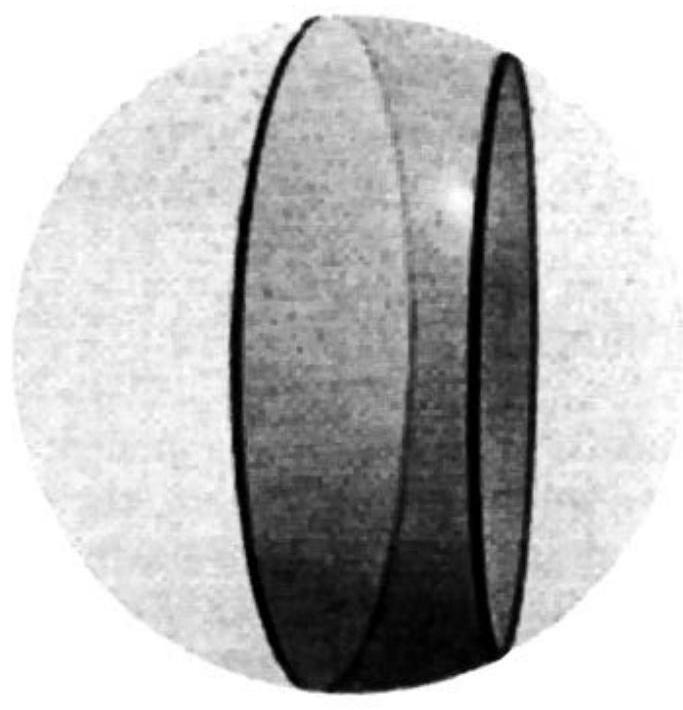
\includegraphics[max width=\textwidth]{2022_11_30_0cbb01a33d99487fc27fg-159}
\end{center}

Figure 3. Sphere distribution integral.

\section{III.6 UNIFORM RANDOM ROTATIONS}
\section{Spatial Rotations}
With these warm-up exercises behind us, we are ready to tackle spatial rotations. Once again there are several possible representations, including Euler angles $\left(\theta_{x^{\prime}}, \theta_{y}, \theta_{z}\right)$, unit quaternions $\mathrm{w}+\mathbf{i v}+\mathbf{j x}+\mathbf{k z}$ (Shoemake, 1985, 1989), and $3 \times 3$ matrices

$$
\begin{array}{ccc}
1-2\left(y^{2}+z^{2}\right) & 2 x y-2 w z & 2 x z+2 w y \\
2 x y+2 w z & 1-2\left(x^{2}+z^{2}\right) & 2 y z-2 w x \\
2 x z-2 w y & 2 y z+2 w x & 1-2\left(x^{2}+y^{2}\right)
\end{array}
$$

In this case, unit quaternions are the best representation, and the geometric problem turns out to be one of generating a point uniformly distributed on a sphere in four dimensions, the quaternion unit sphere $\mathrm{x}^{2}+\mathrm{y}^{2}+\mathrm{z}^{2}+\mathrm{w}^{2}=1$. Composition of a random rotation $\mathrm{X}$ with a given rotation $\mathrm{R}$ is given by multiplication of the corresponding unit quaternions, $q_{R} \forall q_{X}$ Multiplication turns (and/ or reflects) the hypersphere, just as two-dimensional rotation composition turns the unit circle. Nonuniformity in the distribution of $q_{x}$ values on the hypersphere shows up as a change-violating the Haar criterion-when it is turned by composition with some $q_{R}$. Turns around any four-dimensional axis are possible (Shoemake, 1991), so there are no "dead spots" where nonuniformity can hide (except equivalence of $q$ and $-q$, but we avoid that loophole by dealing with magnitudes). So only uniformly distributed unit quaternions correspond to uniformly distributed rotations.

\section{Angles Not Uniform}
The average magnitude of, say, the $\mathrm{w}$ component can be computed in perfect analogy to the spherical case. There, the average $\mathrm{x}$ magnitude was obtained by integrating over a hemisphere (to give only positive values) and dividing by the associated area. Here, we integrate over half the hypersphere, and divide by the corresponding hypersurface measure. There, a circle of radius $\cos \theta$ contributed to each $\mathrm{x}$ value of $\sin \theta$; here, a complete three-dimensional sphere of radius $\cos \theta$ contributes to the $\mathrm{w}$

\section{III.6 UNIFORM RANDOM ROTATIONS}
value of $\sin \theta$. The area of a radius $\mathrm{r}$ sphere is $4 \pi \mathrm{r}^{2}$, while that of a unit hypersphere is $2 \pi^{2}$. Thus, the average magnitude of $\mathrm{w}$ for uniformly distributed unit quaternions is given by

$$
\frac{1}{\pi^{2}} \int^{\pi / 2} 4 \pi \cos ^{2} \theta \sin \theta \mathrm{d} \theta=\frac{4}{3 \pi} \approx 0.4244 .
$$

We are now in a position to prove that a uniformly distributed spatial rotation does not have a uniformly distributed angle. For a unit quaternion, the w component is the cosine of half the angle of rotation. When the angle is uniformly distributed between 0 and $2 \pi$, the average magnitude of $w$ will be $2 / \pi \approx 0.6366$, which exceeds the correct value for a uniform rotation by a factor of $\frac{3}{2}$. Thus, the algorithm in Arvo (1991) cannot generate a uniformly distributed rotation, as claimed.

\section{Uniform Rotations from Gaussians}
Fortunately, it is easy to generate random unit quaternions-and hence rotations-with the correct distribution. Assign to the components of a quaternion the values of four Gaussian distributed independent random variables with mean 0 and any common standard deviation-say, 1. Then the quaternion itself will be Gaussian distributed in four-dimensional space (because of the separability of Gaussians) and can be normalized to give a uniformly distributed unit quaternion (because of the spatial symmetry of Gaussians). Pairs of independent variables with Gaussian distribution can easily be generated using the polar, or Box-Muller, method, which transforms a point uniformly distributed within the unit disk. The Gaussian generation can be folded into the unit quaternion generation to give an efficient algorithm (Knuth, 1981, p. 130).

\section{Subgroup Algorithm}
There is, however, a better way to generate uniform random rotations, an approach that generalizes efficiently to any number of dimensions, and to groups other than rotations. In our case, it reduces to the following simple prescription. Let $\mathrm{X}_{0^{\prime}} \mathrm{X}_{1}$, and $\mathrm{X}_{2}$ be three independent random

\section{III.6 UNIFORM RANDOM ROTATIONS}
variables that are uniformly distributed between 0 and 1. Compute two uniformly distributed angles, $\theta_{1}=2 \pi \mathrm{X}_{1}$ and $\theta_{2}=2 \pi \mathrm{X}_{2^{\prime}}$, and their sines and cosines, $\mathrm{s}_{1}, \mathrm{c}_{1}, \mathrm{~s}_{2}, \mathrm{c}_{2}$. Also compute $\mathrm{r}_{1}=\sqrt{1-\mathrm{X}_{0}}$ and $\mathrm{r}_{2}=\sqrt{\mathrm{X}_{0}}$. Then return the unit quaternion with components $\left[s_{1} r_{1}, c_{1} r_{1}, s_{2} r_{2}, c_{2} r_{2}\right]$. Before comparing the computed distribution with the correct distribution, let us look at how this code can be derived from first principles. As we saw earlier, a uniform plane rotation is easily obtained from a uniform angle between 0 and $2 \pi$. Plane rotations form a subgroup of the group of rotations in space, namely rotations around the $\mathrm{z}$ axis. The cosets of this subgroup are represented by the rotations pointing the $\mathrm{z}$ axis in different directions. By multiplying a uniformly distributed element from the subgroup with a uniformly distributed coset representative, the subgroup algorithm generates a uniformly distributed element of the complete group, as explained below.

To better understand the subgroup algorithm, consider a simpler example. The six permutations of a triangle's vertices form a group. Reversing the triangle generates a two-permutation subgroup $(1,2,3)$ and $(3,2,1)$, for which there are three cosets, $\{(1,2,3),(3,2,1)\},\{(2,3,1),(1,3,2)\}$, and $\{(3,1,2),(2,1,3)\}$, each closed under composition with the subgroup permutations. Uniformly choose one of the cosets; then the combination of a permutation from that coset with a uniformly chosen permutation from the subgroup will be uniform over the whole group. Further examples are given in Diaconis and Shahshahani (1986).

In terms of quaternions, a rotation around $z$ has the form $[0,0, s, c]$, while a rotation pointing $\mathrm{z}$ in an arbitrary direction has the form

\begin{center}
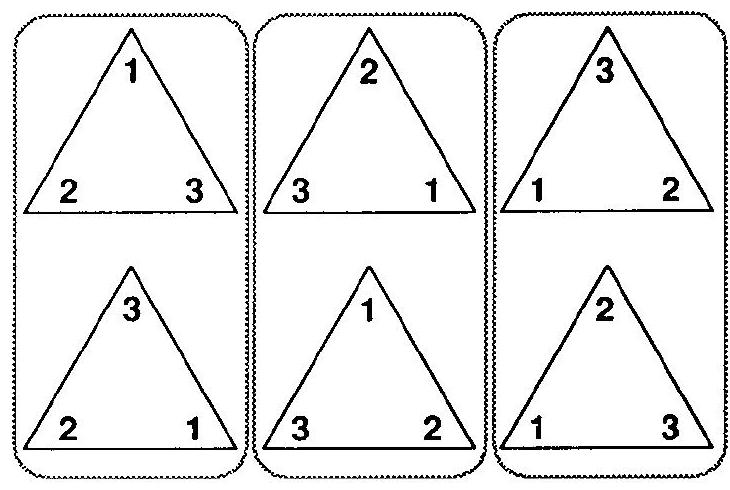
\includegraphics[max width=\textwidth]{2022_11_30_0cbb01a33d99487fc27fg-162}
\end{center}

Figure 4. Cosets in dihedral group.

\section{III.6 UNIFORM RANDOM ROTATIONS}
$[\mathrm{x}, \mathrm{y}, 0, \mathrm{w}]$. If the direction is to be uniformly distributed, w must be distributed as the square root of a uniform distribution, and $\mathrm{x}$ and $\mathrm{y}$ must be a uniform plane rotation times $\sqrt{1-\mathrm{w}^{2}}$. The square root is necessary because the rotated $\mathrm{z}$ value should be uniform for a point uniformly distributed on a sphere. (Remember?) The $\mathrm{z}$ value comes out to be $2 \mathrm{w}^{2}-1$; substituting $\mathrm{w}=\sqrt{\mathrm{X}_{0}}$ gives $2 \mathrm{X}_{0}-1$, a uniform deviate between $-1$ and $+1$, as required. The product of the $\mathrm{z}$ placement with the $z$ rotation is $[c x+s y,-s x+c y, s w, c w]$, which is just one step away from the final code. We know, since this should give points uniformly distributed on a hypersphere, that all components have the same kind of distribution. In particular, the first two components are the product of two uniform plane rotations times a magnitude of $\sqrt{1-X_{0}}$, which can be reduced to a single plane rotation of the correct magnitude, like the last two components. The result is the code stated.

\section{Distribution Check}
Ignoring the derivation, what is the distribution of a component, say, $\sqrt{\mathrm{X}_{0}} \sin \left(2 \pi \mathrm{X}_{2}\right)$ ? The average magnitude can be computed by integrating square root from 0 to 1 , and $1 / \pi$ times the sine from 0 to $\pi$; taking their


\includegraphics[max width=\textwidth, center]{2022_11_30_0cbb01a33d99487fc27fg-163}\\
but not sufficient to show that the distribution is correct, so we press on. The probability that the magnitude of a component is less than or equal to $\mathrm{x}$ should be $2 / \pi\left(\mathrm{x} \sqrt{1-\mathrm{x}^{2}}+\arcsin \mathrm{x}\right)$, a value obtained from

$$
\frac{1}{\pi^{2}} \int_{0}^{\arcsin x}-4 \pi \cos ^{2} \theta d \theta
$$

much as in the spherical case. Obtaining the computed probability is harder. For a uniform distribution, the probability of obtaining a value less than or equal to $\mathrm{x}$ is $F(\mathrm{x})=\mathrm{x}$; for an invertible function $g(\mathrm{x})$ of a uniform distribution, the probability is $\mathrm{F}(\mathrm{x})=\mathrm{g}^{-1}(\mathrm{x})$. Thus, for $\sqrt{\mathrm{X}_{0}}$ we have $F(x)=x^{2}$, while for $\sin \pi / 2 X_{2}$ (with the range restricted for invertibility and magnitude) we have $\mathrm{F}(\mathrm{x})=2 / \pi \arcsin \mathrm{x}$. The density at $\mathrm{x}$ of this latter distribution is the derivative there, $2 / \pi 1 / \sqrt{1-\mathrm{x}^{2}}$. Now

\section{III.6 UNIFORM RANDOM ROTATIONS}
the distribution of the product can be obtained. When the sine term has the value s, the only way to get a product less than or equal to $\mathrm{x}$ is for the square root term to be less than or equal to $\mathrm{x} / \mathrm{s}$, which-since the square root is at most $1-$ has probability $(\operatorname{Min}(\mathrm{x} / \mathrm{s}, 1))^{2}$. Weighting each $\mathrm{s}$ value by its density, and integrating over all s, we have

$$
\begin{aligned}
\int^{1} \frac{2}{\pi} & \frac{1}{\sqrt{1-s^{2}}}(\operatorname{Min}(\mathrm{x} / \mathrm{s}, 1))^{2} \mathrm{ds} \\
&=\int_{1}^{1} \frac{2}{\pi} \frac{1}{\sqrt{1-\mathrm{s}^{2}}}(\mathrm{x} / \mathrm{s})^{2} \mathrm{ds}+\int^{x} \frac{2}{\pi} \frac{1}{\sqrt{1-\mathrm{s}^{2}}} \mathrm{ds} \\
&=\frac{2}{\pi}\left(\mathrm{x} \sqrt{1-\mathrm{x}^{2}}+\arcsin \mathrm{x}\right),
\end{aligned}
$$

as required.

\section{Acknowledgments}
Thanks to James Arvo for his questions and suggestions; this Gem is better as a result.

See also G2, 355; G3, C.4.

\begin{center}
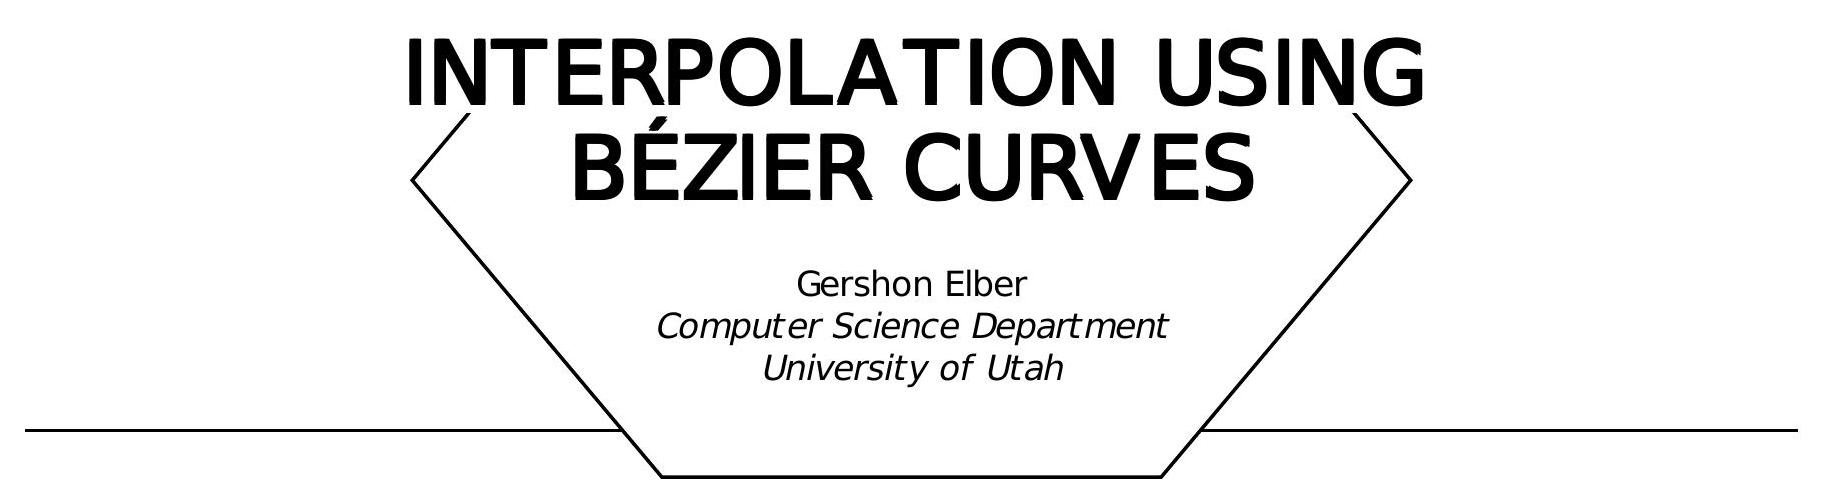
\includegraphics[max width=\textwidth]{2022_11_30_0cbb01a33d99487fc27fg-165}
\end{center}

\section{Introduction}
The Bézier representation (Eq. (1)) is well known and frequently used for CAD applications as it possesses extremely useful properties:

$$
B(t)=\sum_{i=0}^{k} P_{i} B_{i}^{k}(t), \quad B_{i}^{k}(t)={ }_{i}^{k} t^{i}(1-t)^{k-i} .
$$

Bézier curves are easy to evaluate, derive, and subdivide and are unimodal for $t \in[0, \ldots$, 1]. This representation possesses important properties such as control polygon convex hull curve bounding, intuitive curve shape control using control points, and the variation diminishing property. All in all, the Bézier representation is a very useful tool for CAD applications.

A Bézier curve only approximates the shape of its control polygon. If an interpolation scheme is required, this representation cannot usually be used. It may be desired to find the Bézier curve that interpolates a set of points. This will enable the use of the simple and elegant evaluation algorithms (Goldman, 1990) of the Bézier representation with its useful properties.

In this Gem we will present a simple way to find the Bézier curve that interpolates a given set of points.

\section{III.7 INTERPOLATION USING BÉZIER CURVES}
\section{Numeric Solution}
When one attempts to solve the interpolation problem for Bézier curves, a set of linear equations may be defined and solved. Let $\mathbf{B}(\mathrm{t})$ be the Bézier curve interpolating the point set $\mathrm{l}=(\mathbf{T}, \mathbf{V})=\left(\mathrm{t}_{\mathrm{i}}, \mathrm{V}_{\mathrm{i}}\right), \mathrm{i}=0, \ldots, \mathrm{k}, \mathrm{t}, \neq$ $\mathrm{t}_{\mathrm{j}}, \forall \mathrm{i} \neq \mathrm{j}:$

$$
\mathbf{B}\left(\mathrm{t}_{\mathrm{i}}\right)=\mathrm{V}_{\mathrm{i}}, \quad \mathrm{i}=0, \ldots, \mathrm{k}
$$

A one-dimensional Bézier curve of degree $\mathrm{k}$ has $\mathrm{k}+1$ degrees of freedom-its coefficients or control points. Therefore, given a set of $\mathrm{k}+1$ points to interpolate, a Bézier curve of at least degree $\mathrm{k}$ is required to ensure that solution exists.

A linear system of $\mathrm{k}+1$ equations is defined for the $\mathrm{k}+1$ Bézier control polygon points, $\mathbf{P}=\mathrm{P}_{\mathrm{i}}, \mathrm{i}=0, \ldots, \mathrm{k}$, as the unknowns:

$$
\begin{array}{ccccccc}
\mathrm{B}_{0}^{\mathrm{k}}\left(\mathrm{t}_{0}\right) & \mathrm{B}_{1}^{\mathrm{k}}\left(\mathrm{t}_{0}\right) & \cdots & \mathrm{B}_{\mathrm{k}}^{\mathrm{k}}\left(\mathrm{t}_{0}\right) & \mathrm{P}_{0} & = & \mathrm{V}_{0} \\
\mathrm{~B}_{0}^{\mathrm{k}}\left(\mathrm{t}_{1}\right) & \mathrm{B}_{1}^{\mathrm{k}}\left(\mathrm{t}_{1}\right) & \cdots & \mathrm{B}_{\mathrm{k}}^{\mathrm{k}}\left(\mathrm{t}_{1}\right) & \mathrm{P}_{1} & = & \mathrm{V}_{1} \\
\vdots & \vdots & \ddots & \vdots & \vdots & \vdots & \vdots \\
\mathrm{B}_{0}^{\mathrm{k}}\left(\mathrm{t}_{\mathrm{k}}\right) & \mathrm{B}_{1}^{\mathrm{k}}\left(\mathrm{t}_{\mathrm{k}}\right) & \cdots & \mathrm{B}_{\mathrm{k}}^{\mathrm{k}}\left(\mathrm{t}_{\mathrm{k}}\right) & \mathrm{P}_{\mathrm{k}} & = & \mathrm{V}_{\mathrm{k}}
\end{array}
$$

and given input $\mathrm{I}$ one can numerically solve and find $\mathbf{P}$. Note that $\mathrm{V}_{\mathrm{i}}$ (and $P_{i}$ ) may be vectors in which the linear system should be solved coordinatewise. Let $\mathbf{M}$ be the B's square matrix of Eq. (3). As almost all $B_{i}^{k}\left(t_{j}\right) \neq 0$ in $M$, the solution to Eq. (3) is of the order $O\left(k^{3}\right)$ or quite expensive. In the next section we present a way to perform this task without the need to solve such a linear system each time.

\section{Symbolic Solution}
While the numeric technique described in the preceding section is general, one can alleviate the need to solve the linear system each time by posing one more constraint on the problem. Let $\mathrm{l}=\left((\mathrm{i} / \mathrm{k}), \mathrm{V}_{\mathrm{i}}\right), \mathrm{i}=$ $0, \ldots, k$, be the set of points to interpolate. In other words, the parameter value interpolating $\mathrm{V}_{\mathrm{i}}$ is not free any more, but equal to i/k. One only

\section{III.7 INTERPOLATION USING BÉZIER CURVES}
needs to specify $\mathbf{V}$ or $\mathrm{l}=(\mathbf{V})=\left(\mathrm{V}_{\mathrm{i}}\right), \mathrm{i}=0, \ldots, \mathrm{k}$, as now the $t_{\mathrm{i}}$ s are in fixed and equally spaced positions.

$\mathrm{B}_{\mathrm{i}}^{\mathrm{k}}(\mathrm{t})$ maximum is at $\mathrm{i} / \mathrm{k}$. Therefore, $\mathrm{P}_{\mathrm{i}}$ is most influenced from $\mathrm{V}_{\mathrm{i}}$, which is usually more intuitive. However, any fixed and distinguished set of $\mathrm{k}+1$ parameter values may be used in a similar way.

Updating Eq. (3) and using this new constraint, we get

$$
\begin{aligned}
& \mathrm{B}_{0}^{\mathrm{k}} \frac{0}{\mathrm{k}} \quad \mathrm{B}_{1}^{\mathrm{k}} \frac{0}{\mathrm{k}} \quad \cdots \quad \mathrm{B}_{\mathrm{k}}^{\mathrm{k}} \frac{0}{\mathrm{k}} \quad \mathrm{P}_{0}=\mathrm{V}_{0} \\
& \mathrm{B}_{0}^{\mathrm{k}} \frac{1}{\mathrm{k}} \quad \mathrm{B}_{1}^{\mathrm{k}} \frac{1}{\mathrm{k}} \quad \cdots \quad \mathrm{B}_{\mathrm{k}}^{\mathrm{k}} \frac{1}{\mathrm{k}} \quad \mathrm{P}_{1}=\mathrm{V}_{1} \text {. } \\
& \mathrm{B}_{0}^{\mathrm{k}} \frac{\mathrm{k}}{\mathrm{k}} \quad \mathrm{B}_{1}^{\mathrm{k}} \frac{\mathrm{k}}{\mathrm{k}} \quad \cdots \quad \mathrm{B}_{\mathrm{k}}^{\mathrm{k}} \frac{\mathrm{k}}{\mathrm{k}} \quad \mathrm{P}_{\mathrm{k}} \quad=\quad \mathrm{V}_{\mathrm{k}}
\end{aligned}
$$

Interestingly enough, $\mathbf{M}$ in Eq. (4) is independent of $\mid$. In other words, one can solve this system (invert M) without knowing anything about the input set I ! Given a set of points, I, the control polygon of the Bézier curve interpolating $\mid$ is

$$
\mathbf{P}=\mathbf{M}^{-1} \mathbf{V},
$$

where $\mathbf{M}^{-1}$ is $\mathbf{M}$ inverse.

By picking i/ $\mathrm{k}$ as the parameters at which the Bézier curve is interpolating the input data, all the terms in $\mathbf{M}, \mathrm{M}_{\mathrm{ji}}$, are of the form

\begin{center}
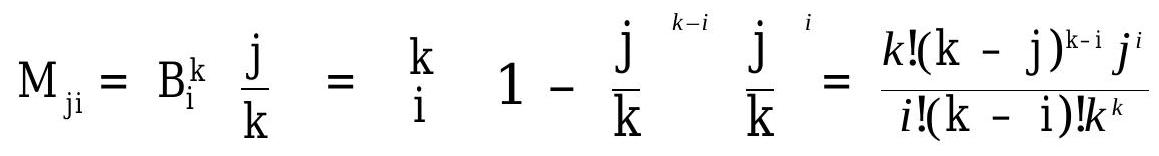
\includegraphics[max width=\textwidth]{2022_11_30_0cbb01a33d99487fc27fg-167}
\end{center}

or the term in Eq. (6) and therefore all the terms in $\mathbf{M}$ and $\mathbf{M}^{-1}$ may be expressed as rational integers exactly.

\section{III.7 INTERPOLATION USING BÉZIER CURVES}
\section{Implement ation}
The C program provided uses the symbolic solution for $\mathbf{M}^{-1}$ for Bézier curves from order 2 (linear) to 9. A long rational integer (32 bits) is used to hold the exact symbolic solution (Reduce, 1987). The zero element of each row holds the line common denominator for the rest of the line numerators. Most of the implementation is, in fact, the symbolic solution represented as rational values. The following routines simply multiply this matrix solution by the given $\mathbf{V}$ input set to find the control polygon point set, P.

See also G1, 75; G3, C.4.\\

\includegraphics[max width=\textwidth, center]{2022_11_30_0cbb01a33d99487fc27fg-169}

Superquadric ellipsoids and toroids are recent geometric shapes, useful for computer graphics modeling. In this article, we provide equations needed to calculate the motion of these shapes in rigid physically based modeling: We present closed-form algebraic expressions for the volume, center of mass, and rotational inertia tensor for (constant density) superquadric shapes. We do not cover nonrigid physically based motion. In the appendices, we briefly review superquadrics, the equations of rigid body motion of Newtonian physics, and ancillary mathematical definitions and derivations.

\section{Review of Superquadrics}
Superquadrics (Barr, 1981) are three-dimensional extensions of Piet Hein's two-dimensional superellipses (Faux and Pratt, 1979). They allow us to easily represent rounded, square, cylindrical, pinched, and toroidal shapes with relatively simple equations. The superquadric parametric surface function is a profile surface based on trigonometric functions raised to exponents (which retain the appropriate plus or minus sign in their octant).

There are six shape parameters of the superquadrics:

\begin{itemize}
  \item the roundness/ squareness shape parameter in the north-south direction is " $\mathrm{n}$ "
\end{itemize}

\section{III.8 RIGID PHYSICALLY BASED SUPERQUADRICS}
\begin{center}
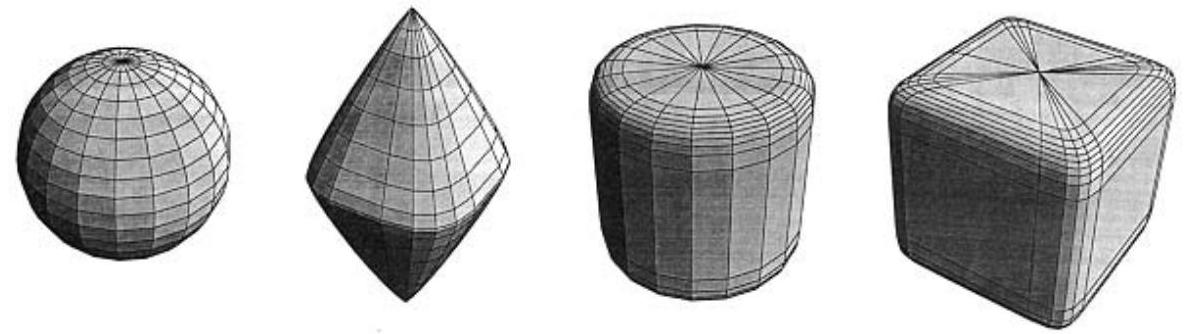
\includegraphics[max width=\textwidth]{2022_11_30_0cbb01a33d99487fc27fg-170}
\end{center}

Figure 1. Examples of superquadric ellipsoids. From left to right, we produce a sphere, a pyramid, a cylindroid, and a cuboid. The north-south parameters, respectively, are 1.0, $1.8,0.2,0.2$, and the east-west parameters are 1.0, 0.6, 1.0, and 0.2.

\begin{itemize}
  \item the east-west roundness/ squareness parameter is " $\mathrm{e}^{\text {" }}$

  \item $\mathrm{a}_{1}, \mathrm{a}_{2}$, and $\mathrm{a}_{3}$ are length, width, and depth parameters

  \item for toroids, " $\alpha$ " is a "hole diameter" parameter and should be greater than one, to avoid self-intersection.

\end{itemize}

Equations reviewing the geometric properties of superquadrics are found in Appendix A.

\section{Rigid Physically Based Superquadric Quantities}
We need several quantities to calculate physically based computer graphics motions of rigid bodies. Specifically, we need to know

\begin{enumerate}
  \item the position $\mathrm{x}_{\mathrm{C}}$ of the center of mass of the object,

  \item the net mass $M$ of the bodies, and

  \item the rotational inertia tensor, $\underline{\underline{I}}$, of the body.

\end{enumerate}

We use these quantities in the equations of rigid body motion, which we review briefly in Appendix B. We use notation similar to that of Barzel and Barr (1988) and refer the reader to that article and to Barzel (1992) for a description of rigid body motion and methods to calculate dynamic constraints on rigid bodies. We refer to Barr (1984), Terzopoulis et al. (1987), and Pentland and Williams (1989) for different types of nonrigid motion.

\section{III.8 RIGID PHYSICALLY BASED SUPERQUADRICS}
\begin{center}
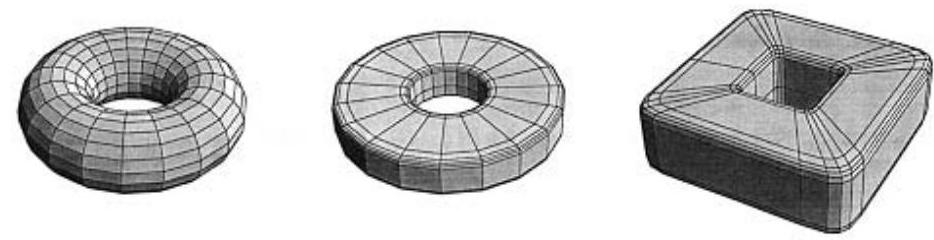
\includegraphics[max width=\textwidth]{2022_11_30_0cbb01a33d99487fc27fg-171}
\end{center}

Figure 2. Examples of superquadric toroids. From left to right, we produce a round torus, a "pineapple-slice" toroid, and a square toroid. The north-south parameters, respectively, are 1.0, 0.2, 0.2, and the east-west parameters are 1.0, 1.0, and 0.2. The hole parameter, $\alpha$, is 2.

\section{Center of Mass}
For the canonical superquadrics described in Appendix A, the position of the center of mass is at the origin:

$$
\underline{\mathrm{x}}_{C}=\underline{0} .
$$

Of course, when we calculate a new center of mass of the object from the equations of rigid body motion, we need to translate the superquadric to the new position.

\section{Volume, Density, and Mass}
There are a number of ways to specify volume, density, and mass. In this article, we let the terms $\rho$ and $\mathrm{M}$ be the density and mass of the superquadric object (ellipsoid or toroid). The user first chooses the substance of the object (say steel or wood), which determines $\rho$, its density. Then the mass of the object is determined from the object's volume. 1

We let $V_{E}$ signify the volume of the superquadric ellipsoids, and $V_{T}$ the volume of the toroids (V without either subscript can signify the volume of either shape). We express the volume formula in terms of beta functions, $\beta(\mathrm{m}, \mathrm{n})$. Methods for computing $\beta(\mathrm{m}, \mathrm{n})$ are shown in Appendix C. Appendix D provides a sketch of the derivation of the volume and inertia tensor formulas.

'This is the recommended approach. Of course, we could also choose the mass first, without choosing a "real" material. Then the density would be the derived quantity, instead of the mass.

\section{III.8 RIGID PHYSICALLY BASED SUPERQUADRICS}
Volume, Superquadric Ellipsoids

$$
\mathrm{V}_{\mathrm{E}}=\frac{2}{3} \mathrm{a}_{1} \mathrm{a}_{2} \mathrm{a}_{3} \mathrm{e} \mathrm{n} \beta \frac{\mathrm{e}}{2}, \frac{\mathrm{e}}{2} \beta \mathrm{n}, \frac{\mathrm{n}}{2} \text {. }
$$

Volume, Superquadric Toroids

$$
\mathrm{V}_{\mathrm{T}}=2 \mathrm{a}_{1} \mathrm{a}_{2} \mathrm{a}_{3} \alpha \mathrm{e} \beta \frac{\mathrm{e}}{2}, \frac{\mathrm{e}}{2} \beta \frac{\mathrm{n}}{2}, \frac{\mathrm{n}}{2} .
$$

Mass, Ellipsoid or Toroid

The mass $\mathrm{M}$ is expressed in terms of the volume $\mathrm{V}$ and density $\rho$. $\rho=$ substance density, $M=\rho V$, where $V$ is the volume of either ellipsoid or toroid.

\section{Inertia Tensor}
The formulas for the inertia tensor are the primary results of this paper. We let $\underline{\underline{I}}_{\mathrm{E}}$ be the inertia tensor of the superquadric ellipsoids, and $\underline{\underline{I}}_{\mathrm{T}}$ the inertia tensor of the toroids.

Inertia Tensor, Superquadric Ellipsoid

In body coordinates, the components of the inertia tensor are constant. The off-diagonal components are zero, due to symmetry arguments:

$$
\begin{aligned}
& \text { where } \\
& \rho_{\mathrm{E}}=(\text { constant) density of superquadric ellipsoid, } \\
& \mathrm{i}_{1 \mathrm{E}}=\frac{2}{5} \mathrm{a}_{1}^{3} \mathrm{a}_{2} \mathrm{a}_{3} \mathrm{e} \beta 3 \frac{\mathrm{e}}{2}, \frac{\mathrm{e}}{2} \beta 2 \mathrm{n}, \frac{\mathrm{n}}{2} \text {, } \\
& \mathrm{i}_{2 \mathrm{E}}=\frac{2}{5} \mathrm{a}_{1} \mathrm{a}_{2}^{3} \mathrm{a}_{3} \mathrm{e} \mathrm{n} \beta \frac{\mathrm{e}}{2}, 3 \frac{\mathrm{e}}{2} \beta 2 \mathrm{n}, \frac{\mathrm{n}}{2} \text {, } \\
& \mathrm{i}_{3 \mathrm{E}}=\frac{2}{5} \mathrm{a}_{1} \mathrm{a}_{2} \mathrm{a}_{3}^{3} \mathrm{e} \mathrm{n} \beta \frac{\mathrm{e}}{2}, \frac{\mathrm{e}}{2} \beta \mathrm{n}, \frac{3 \mathrm{n}}{2} \text {. }
\end{aligned}
$$

\begin{center}
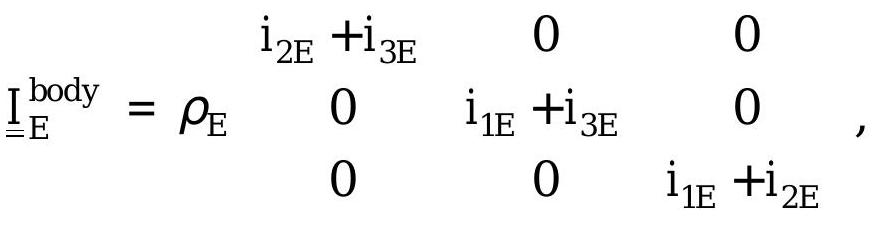
\includegraphics[max width=\textwidth]{2022_11_30_0cbb01a33d99487fc27fg-172}
\end{center}

\section{III.8 RIGID PHYSICALLY BASED SUPERQUADRICS}
In Appendix $D$, we show the derivation of $i_{1 E^{\prime}} i_{2 E^{\prime}}$ and $i_{3 E^{\prime}}$ along with the volume, V.

\section{Inertia Tensor, Superquadric Toroid}
Likewise, the components of the toroid inertia tensor are constant in body coordinates.

$$
\begin{aligned}
& \mathrm{i}_{2 \mathrm{~T}}+\mathrm{i}_{3 \mathrm{~T}} \quad 0 \quad 0 \\
& \underline{\underline{I}}_{\mathrm{T}}^{\text {body }}=\rho_{\mathrm{T}} \quad \begin{array}{lllll} & \mathrm{i}_{1 \mathrm{~T}}+\mathrm{i}_{3 \mathrm{~T}} & 0 & \text { where }\end{array} \\
& \begin{array}{lll}0 & 0 & \mathrm{i}_{1 \mathrm{~T}}+\mathrm{i}_{2 \mathrm{TT}}\end{array} \\
& \rho_{\mathrm{T}}=\text { (constant) density of superquadric toroid, } \\
& \mathrm{i}_{1 \mathrm{~T}}=\mathrm{a}_{1}^{3} \mathrm{a}_{2} \mathrm{a}_{3} \alpha \mathrm{en} \beta 3 \frac{\mathrm{e}}{2}, \frac{\mathrm{e}}{2} \quad 2 \alpha^{2} \beta \frac{\mathrm{n}}{2}, \frac{\mathrm{n}}{2}+3 \beta \frac{3 \mathrm{n}}{2}, \frac{\mathrm{n}}{2} \text { , } \\
& \mathrm{i}_{2 \mathrm{~T}}=\mathrm{a}_{1} \mathrm{a}_{2}^{3} \mathrm{a}_{3} \alpha \mathrm{e} \beta \frac{\mathrm{e}}{2}, 3 \frac{\mathrm{e}}{2} \quad 2 \alpha^{2} \beta \frac{\mathrm{n}}{2}, \frac{\mathrm{n}}{2}+3 \beta \frac{3 \mathrm{n}}{2}, \frac{\mathrm{n}}{2} \text {, } \\
& \mathrm{i}_{3 \mathrm{~T}}=\mathrm{a}_{1} \mathrm{a}_{2} \mathrm{a}_{3}^{3} \alpha \mathrm{n} \beta \frac{\mathrm{e}}{2}, \frac{\mathrm{e}}{2} \beta \frac{\mathrm{n}}{2}, \frac{3 \mathrm{n}}{2} \text {. }
\end{aligned}
$$

In Appendix D, we show the derivation of $i_{1 T}, i_{2 T^{\prime}}$ and $i_{3 T^{\prime}}$ along with the volume, V.

\section{Examples of the Volume and Inertia Tensors}
For some values of $\mathrm{n}$ and e, the superquadric inertia tensor is particularly simple and can be compared to known inertia tensors of spheres, ellipsoids, blocks, and cones. Note that the values of $a_{1}, a_{2}$, and $a_{3}$ are the principal radii of the shapes (not the diameters!).

\section{Superquadric Ellipsoid Examples}
We present the volume and nonzero components of the inertia tensors for particular superquadric ellipsoids. The reader can compare the results of their numerical computations to these formulas, for verification purposes.

\section{III.8 RIGID PHYSICALLY BASED SUPERQUADRICS}
\begin{center}
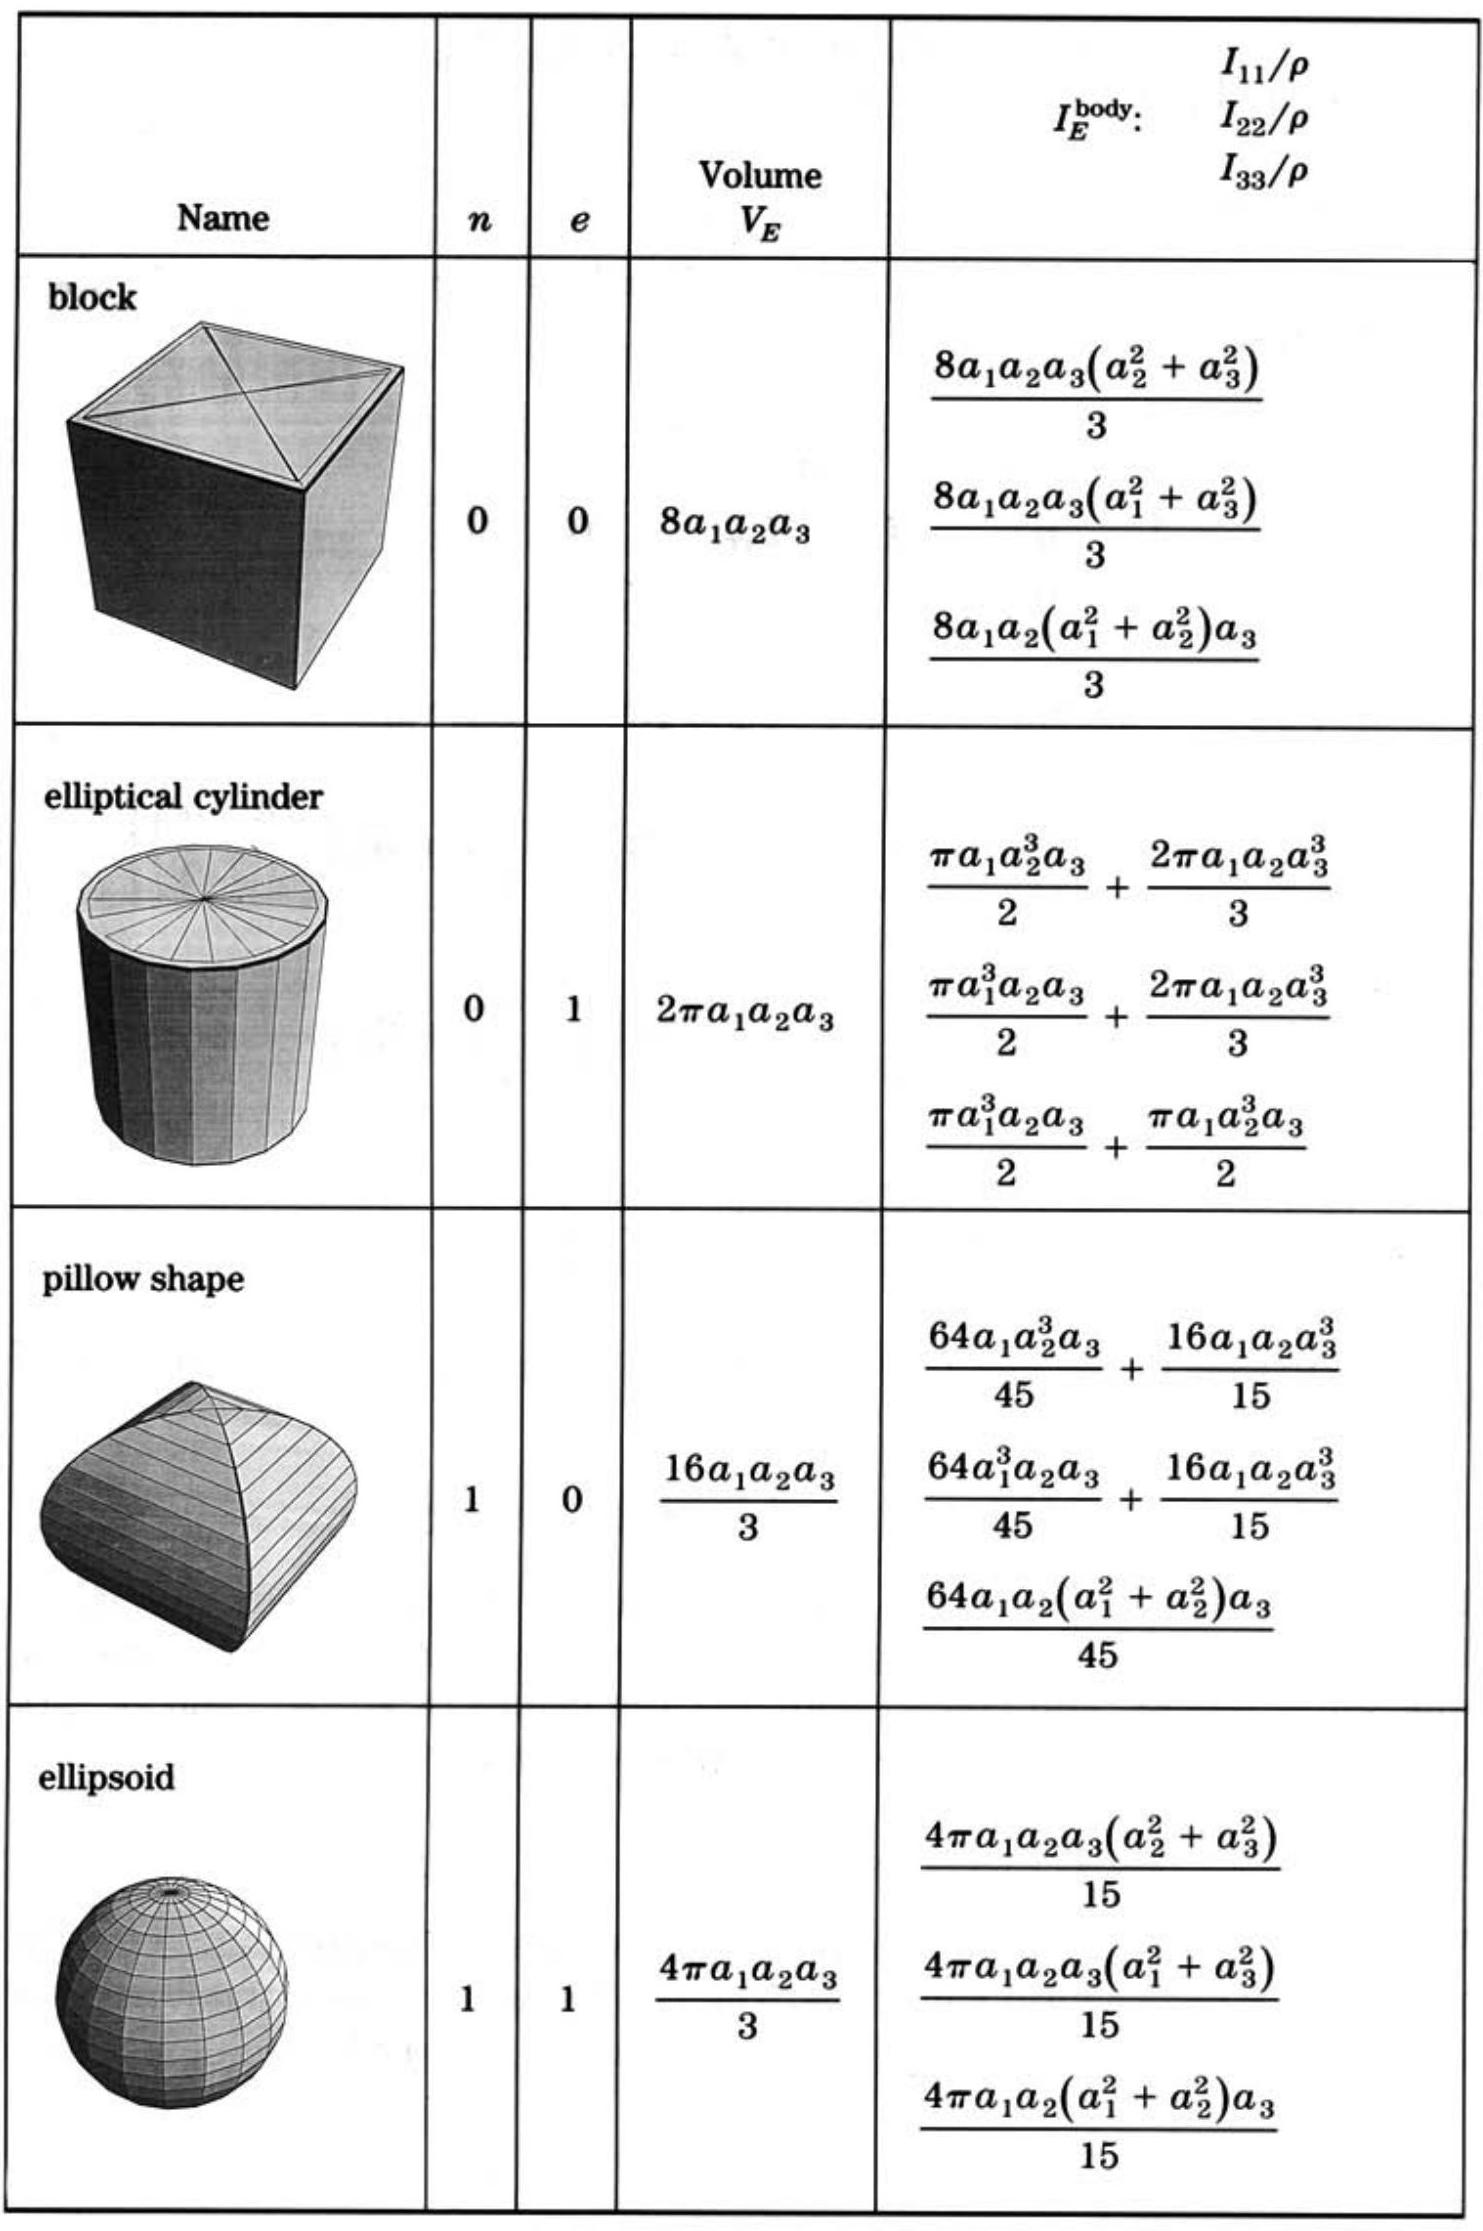
\includegraphics[max width=\textwidth]{2022_11_30_0cbb01a33d99487fc27fg-174}
\end{center}

\section{III.8 RIGID PHYSICALLY BASED SUPERQUADRICS}
\begin{center}
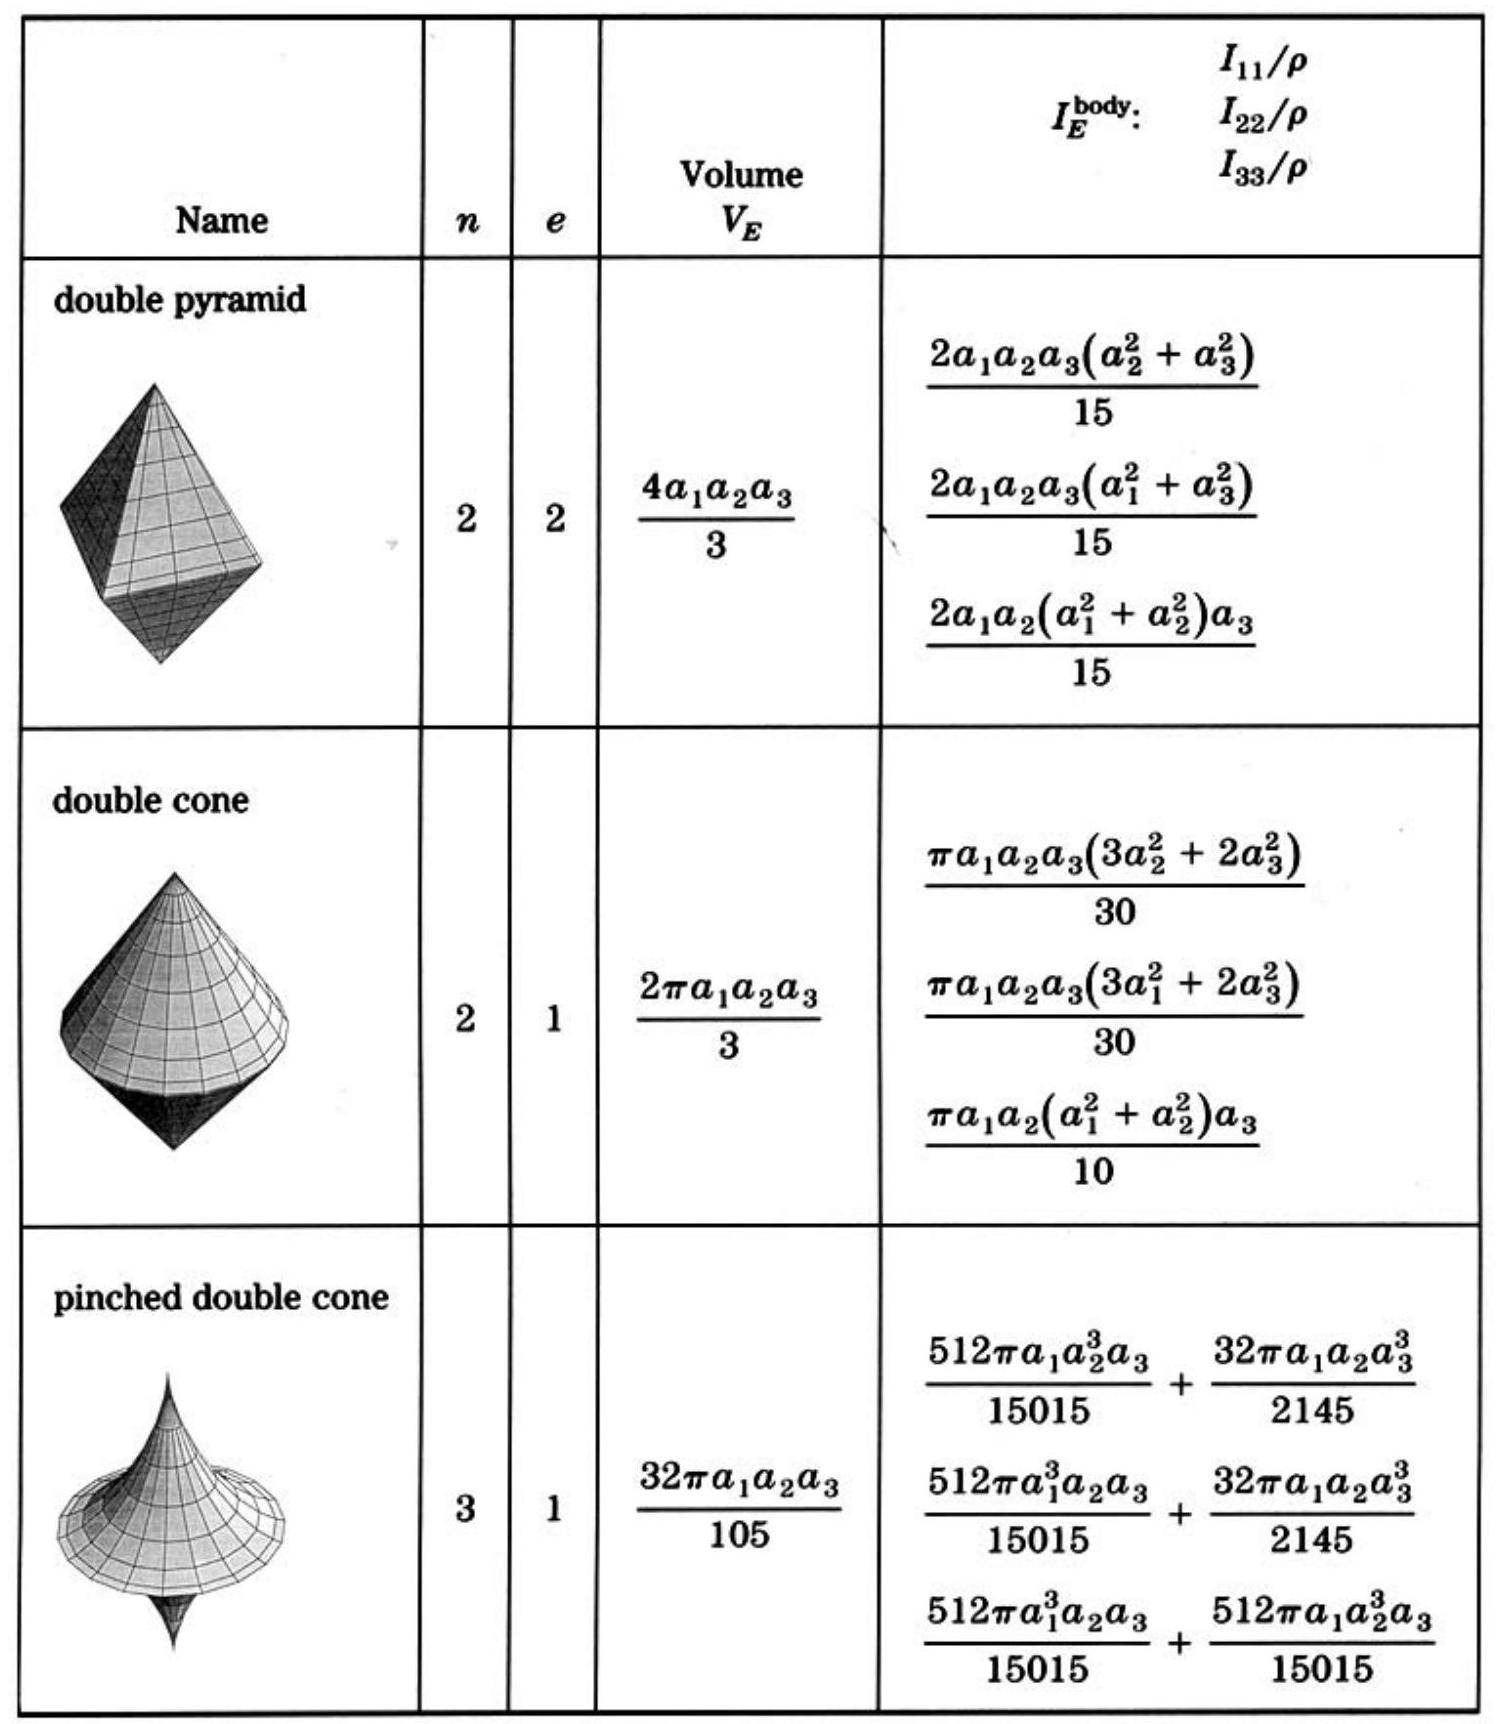
\includegraphics[max width=\textwidth]{2022_11_30_0cbb01a33d99487fc27fg-175}
\end{center}

\section{Toroid Examples}
We provide similar test cases for the superquadric toroids.

\section{III.8 RIGID PHYSICALLY BASED SUPERQUADRICS}
\begin{center}
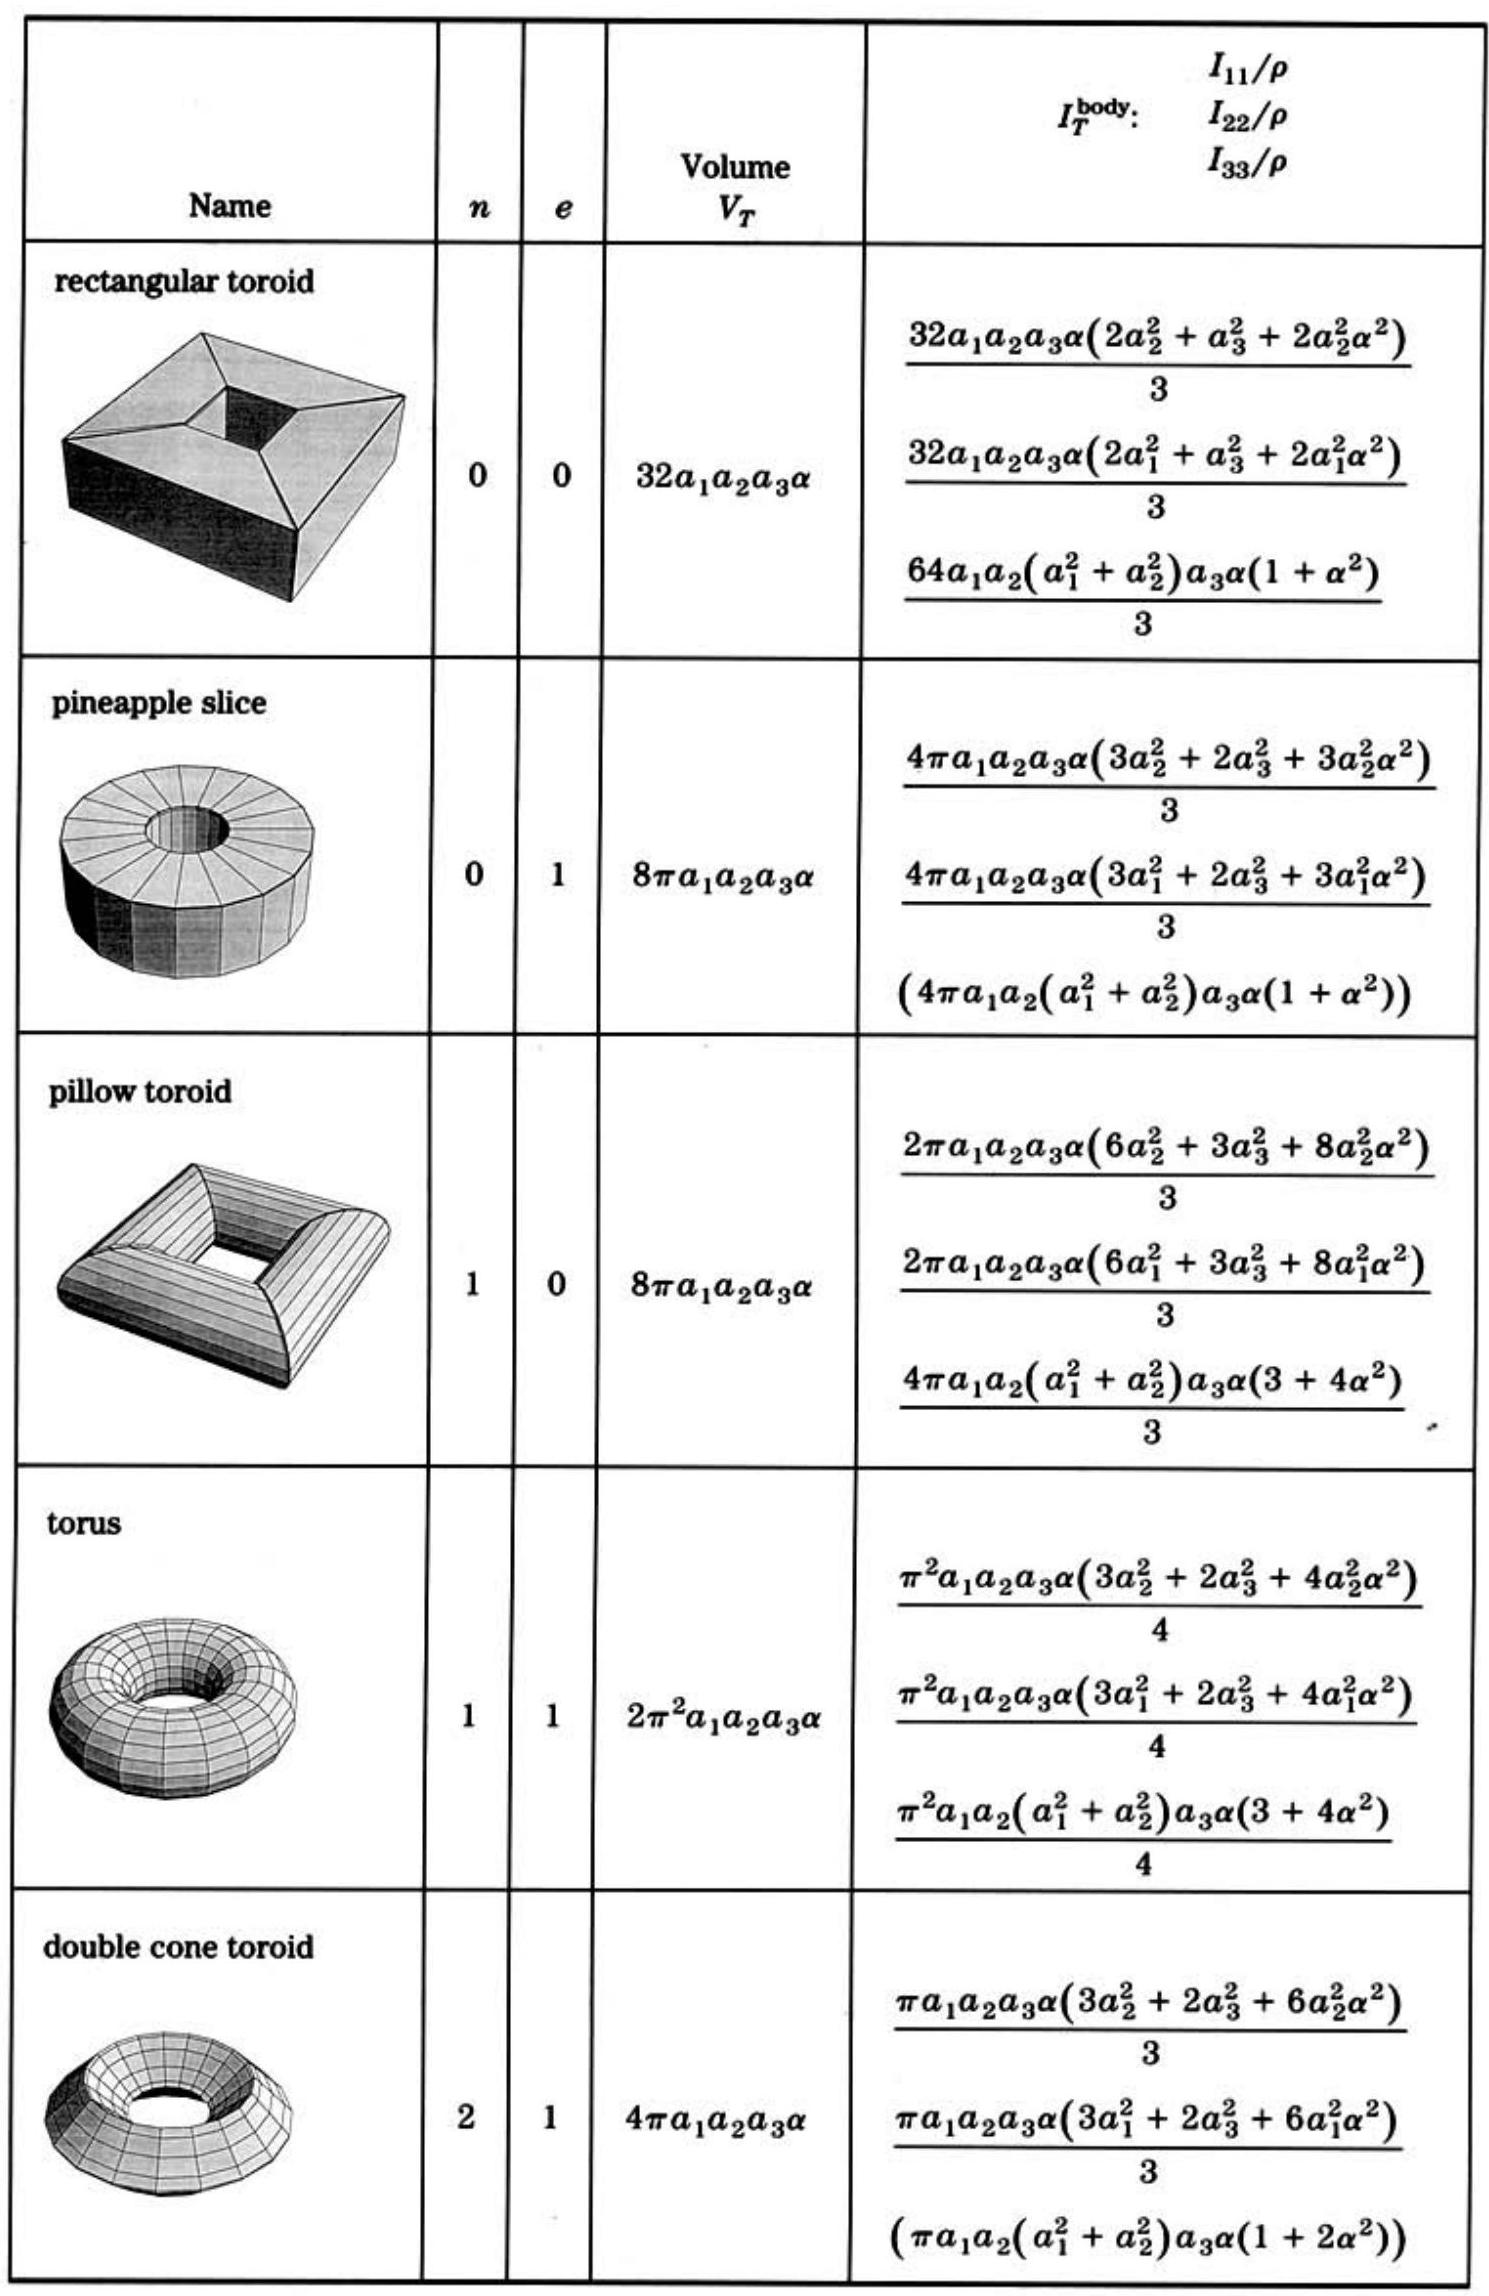
\includegraphics[max width=\textwidth]{2022_11_30_0cbb01a33d99487fc27fg-176}
\end{center}

\section{III.8 RIGID PHYSICALLY BASED SUPERQUADRICS}
\section{Obtaining the Tensors and Their Inverses in World Coordinates}
To obtain the components of the inertia tensor in world coordinates, we use the same $3 \times 3$ rotation matrix $\underline{\underline{\mathrm{R}}}$ that rotates the body vectors into world coordinates.

The inertia tensor in world coordinates is given by

$$
\left(I^{\text {world }}\right)_{\mathrm{ij}}=\sum_{\mathrm{k}=1}^{3} \sum_{=1}^{3} \mathrm{R}_{\mathrm{ik}} \mathrm{R}_{\mathrm{jl}}\left(\mathrm{I}^{\text {body }}\right)_{\mathrm{kl}} .
$$

The components of the inverse matrix of the inertia tensor in world coordinates are given by

$$
\left(\left(I^{\text {world }}\right)^{-1}\right)_{\mathrm{ij}}=\sum_{\mathrm{k}=1}^{3} \sum_{=1}^{3} R_{\mathrm{ik}} \mathrm{R}_{\mathrm{j} l}\left(\left(I^{\text {body }}\right)^{-1}\right)_{\mathrm{kl}} .
$$

Note that in the body coordinate system, the components of the matrices are constant and only need to be computed once (and that in world coordinates the components change as a function of time).

\section{Conclusion}
By applying the results of the preceding sections in the context of Appendix B, the reader is able to add superquadric shapes to a previously written physically based computer graphics modeling package.

\section{Acknowledgment}
I would like to thank Dr. John Snyder for alternate numerical computations used to double-check the closed-form equations for volume and inertia tensor.

\section{III.8 RIGID PHYSICALLY BASED SUPERQUADRICS}
\section{Appendix A: Review of Superquadric Geometric Quantities}
Superquadrics have an unusual property: They have closed-form algebraic expressions for their most important geometric features. This closed-form property makes them easier to use and more appropriate for computer graphics applications. Thus, like spheres, they have

\begin{enumerate}
  \item a relatively simple parametric form of their surface,

  \item an implicit function to test if a given 3-D point is inside or outside of the shape, and

  \item simple expressions for their normal vectors.

\end{enumerate}

\section{Parametric Surface Functions}
We need three functions, $\mathrm{c}(\mathrm{w}, \mathrm{m}), \mathrm{s}(\mathrm{w}, \mathrm{m})$, and $\mathrm{c}_{\mathrm{T}}(\mathrm{w}, \mathrm{m}, \alpha)$ to calculate the parametric surface for superquadric ellipsoids and toroids:

$$
\begin{gathered}
\mathrm{c}(\mathrm{w}, \mathrm{m})=\operatorname{sgn}(\cos (\mathrm{w}))|\cos (\mathrm{w})|^{\mathrm{m}}, \\
\mathrm{c}_{\mathrm{T}}(\mathrm{w}, \mathrm{m}, \alpha)=\alpha+\mathrm{c}(\mathrm{w}, \mathrm{m}), \quad \alpha>1, \\
\mathrm{~s}(\mathrm{w}, \mathrm{m})=\operatorname{sgn}(\sin (\mathrm{w}))|\sin (\mathrm{w})|^{\mathrm{m}} .
\end{gathered}
$$

For us,

$$
\begin{aligned}
& -1, \quad \mathrm{x}<0 \\
& \operatorname{sgn}(\mathrm{x})=0, \quad \mathrm{x}=0 . \\
& 1, \mathrm{x}>0
\end{aligned}
$$

Also, note that $\mathrm{c}_{\mathrm{T}}(\mathrm{w}, \mathrm{m}, \alpha)$ is always greater than zero (to avoid self-intersection).

\section{III.8 RIGID PHYSICALLY BASED SUPERQUADRICS}
\section{Superquadric Ellipsoid}
(Surface parameters $u$ and $v$; dimensions: $a_{1}, a_{2}, a_{3} ;$ roundness/ squareness shape parameters: $n$, e.)

$$
\begin{gathered}
\mathrm{x}(u, v)=a_{1} c(v, n) c(u, e) \\
y(u, v)=a_{2} c(v, n) s(u, e) \\
z(u, v)=a_{3} s(v, n) \\
-\pi / 2 \leq v \leq \pi / 2, \quad-\pi \leq u<\pi .
\end{gathered}
$$

See Figs. 1 and 3.

\section{Superquadric Toroid}
(Surface parameters $u$ and $v$; dimension parameters: $a_{1}, a_{2}, a_{3}$; hole diameter parameter: $\alpha, \alpha>1$; roundness/ squareness shape parameters: n, e.)

$$
\begin{aligned}
& \mathrm{x}(\mathrm{u}, \mathrm{v})=\mathrm{a}_{1} \mathrm{C}_{\mathrm{T}}(\mathrm{v}, \mathrm{n}, \alpha) \mathrm{c}(\mathrm{u}, \mathrm{e}), \\
& y(u, v)=a_{2} c_{T}(v, n, \alpha) s(u, e), \\
& z(u, v)=a_{3} s(v, n), \\
& -\pi \leq \mathrm{v}<\pi, \quad-\pi \leq \mathrm{u}<\pi .
\end{aligned}
$$

Note that unlike the ellipsoids, the $\mathrm{v}$ parameter for the toroids goes completely around a circle, from $-\pi$ to $\pi$, instead of only halfway around.

See Figs. 2 and 4.

\section{"Inside-Outside" Function}
If $f(x, y, z)<0$ we are inside the object; if $f(x, y, z)=0$ we are on the object, while if $f(x, y, z)>0$ we are outside the object.

\section{III.8 RIGID PHYSICALLY BASED SUPERQUADRICS}
\section{"Inside-Outside" Function of Superquadric Ellipsoids}
$$
\mathrm{f}(\mathrm{x}, \mathrm{y}, \mathrm{z})=\left(\left|\mathrm{x} / \mathrm{a}_{1}\right|^{2 / \mathrm{e}}+\left|\mathrm{y} / \mathrm{a}_{2}\right|^{2 / \mathrm{e}}\right)^{\mathrm{e} / \mathrm{n}}+\left|\mathrm{z} / \mathrm{a}_{3}\right|^{2 / \mathrm{n}}-1
$$

\section{"Inside-Outside" Function of Superquadric Toroids}
$$
\mathrm{f}(\mathrm{x}, \mathrm{y}, \mathrm{z})=\left|\left(\left|\mathrm{x} / \mathrm{a}_{1}\right|^{2 / \mathrm{e}}+\left|\mathrm{y} / \mathrm{a}_{2}\right|^{2 / \mathrm{e}}\right)^{e / 2}-\alpha\right|^{2 / \mathrm{n}}+\left|\mathrm{z} / \mathrm{a}_{3}\right|^{2 / \mathrm{n}}-1
$$

\section{Normal Vectors}
As the reader is aware of, normal vectors are used in computer graphics shading operations. To obtain unit normal vectors, you need to divide by the magnitude of the normal vectors in the following equations:

Normal Vectors, Superquadric Ellipsoids and Toroids, Parametric Form

$$
\begin{aligned}
&N_{1}(u, v)=\frac{1}{a_{1}} c(v, 2-n) c(u, 2-e), \\
&N_{2}(u, v)=\frac{1}{a_{2}} c(v, 2-n) s(u, 2-e), \\
&N_{3}(u, v)=\frac{1}{a_{3}} s(v, 2-n) .
\end{aligned}
$$

Normal Vectors, Superquadric Ellipsoids and Toroids, Implicit Form

$$
\begin{aligned}
&N_{1}=\frac{\partial f(x, y, z)}{\partial x}, \\
&N_{2}=\frac{\partial f(x, y, z)}{\partial y}, \\
&N_{3}=\frac{\partial f(x, y, z)}{\partial z} .
\end{aligned}
$$

\section{III.8 RIGID PHYSICALLY BASED SUPERQUADRICS}
\section{Appendix B: Some Equations of Rigid-Body Motion}
Although we cannot provide a complete description of rigid-body motion within the scope of this article, we can review parts of it briefly.

The main purpose of the rotational inertia tensor $\underline{\underline{I}}$ is to allow us to convert between angular momentum $\underline{L}$ and angular velocity $\underline{\omega}$. The rotational inertia matrix times the angular velocity is the angular momentum. It is very similar to the conversion between linear momentum $\underline{P}$ and linear velocity $\underline{\mathrm{v}}$. The mass (linear inertia) $\mathrm{M}$ times the velocity is the linear momentum $\underline{P}$.

There are several types of equations that rigid-body motion utilizes:

Differential equations:

$$
\begin{aligned}
\underline{\mathrm{x}}^{\mathrm{\prime}} &=\underline{\mathrm{v}}, \\
\underline{\mathrm{q}}_{\mathrm{i}}^{\prime} &=\frac{1}{2}-\omega \cdot \mathrm{r} \\
\underline{\mathrm{P}}^{\prime} &=\mathrm{F} \omega+\omega \times \mathrm{r} \\
\underline{\mathrm{P}}^{\prime} &=\mathrm{T} ;
\end{aligned}
$$

\section{Initial conditions:}
$$
\begin{aligned}
&\underline{\mathrm{x}}(0)=\underline{\mathrm{x}}_{0}, \\
&\underline{\mathrm{q}}(0)=\underline{\mathrm{q}}_{0^{\prime}} \\
&\underline{\mathrm{P}}(0)=\mathrm{M}_{\underline{\mathrm{v}}_{0}}, \\
&\underline{\mathrm{L}}(0)=\underline{\underline{\mathrm{I}}}^{\text {world }} \underline{\omega}_{0} ;
\end{aligned}
$$

\section{III.8 RIGID PHYSICALLY BASED SUPERQUADRICS}
Auxiliary equations:

$$
\begin{aligned}
& \underline{v}=\frac{P}{M} \text {, } \\
& \underline{\omega}=\left(\underline{\underline{I}}^{\text {world }}\right)^{-1} \mathrm{~L}, \\
& 1-2 \hat{q}_{2}^{2}-2 \hat{q}_{3}^{2} \quad 2 \hat{q}_{1} \hat{q}_{2}-2 \hat{q}_{0} \hat{q}_{3} \quad 2 \hat{q}_{1} \hat{q}_{3}+2 \hat{q}_{2} \hat{q}_{3} \\
& \underline{\underline{R}}=2 \hat{q}_{1} \hat{q}_{2}+2 \hat{q}_{0} \hat{q}_{3} \quad 1-2 \hat{q}_{1}^{2}-2 \hat{q}_{3}^{2} \quad 2 \hat{q}_{2} \hat{q}_{3}-2 \hat{q}_{0} \hat{q}_{1} \\
& 2 \hat{q}_{1} \hat{q}_{3}-2 \hat{q}_{0} \hat{q}_{1} \quad 2 \hat{q}_{2} \hat{q}_{3}+2 \hat{q}_{0} \hat{q}_{1} \quad 1-2 \hat{q}_{1}^{2}-2 \hat{q}_{2}^{2} \\
& s \text { = scalar part of quaternion } \\
& \mathrm{r}=\text { vector part of quaternion }
\end{aligned}
$$

where

$\underline{\mathrm{x}}$ is a three-by-one vector for the position of the center of mass of the object, for us to translate our object by;

$\underline{\underline{R}}$ is a right-handed three-by-three rotation matrix that rotates the object;

$\underline{P}$ is the linear momentum of the object (a three-by-one vector);

$\mathrm{L}$ is the angular momentum of the object (three-by-one vector);

$\underline{F}$ is the net force acting on the object's center of mass (a three-by-one vector);

T is the net torque acting around the object's center of mass (a three-by-one vector);

$\underline{v}$ is the linear velocity of the object (a three-by-one vector);

$\underline{\omega}$ is the angular velocity of the object (a three-by-one vector);

$\mathrm{M}$ is the mass of the object;

$\underline{\underline{I}}^{\text {world }}$ is a three-by-three matrix for the rotational inertia tensor of the object in world coordinates (see the section in the text on the inertia tensor);

and $\hat{q}=q / \sqrt{q \cdot q}$

Please see Goldstein (1980) for additional details.

\section{III.8 RIGID PHYSICALLY BASED SUPERQUADRICS}
\section{Appendix C: How to Compute $\beta(m, n)$, and $\Gamma(n)$ 
 Integral Form of the Beta Function}
The $\beta$ function is defined via the integral

$$
\int_{0}^{1} t^{n-1}(1-t)^{\mathrm{m}-1} d t=\beta(m, n) .
$$

The parameters $\mathrm{m}$ and $\mathrm{n}$ are nonnegative real numbers.

The volume and inertia tensor derivation is based on the following integral, where we transform the preceding definition. We let $\mathrm{t}=\sin ^{2}(\mathrm{x})$ and divide both sides by 2 :

$$
\int_{0}^{\pi / 2} \cos ^{2 n-1}(x) \sin ^{2 m-1}(x) d x=\frac{1}{2} \beta(m, n) .
$$

Thus, we can evaluate any definite integral with an integrand consisting of $\sin$ and cos raised to (non-integer) powers (if we can coerce it into having limits from zero to $\pi / 2$ ). This is the heart of the derivation shown in Appendix D.

\section{How to Compute $\beta(n, m)$}
When we wish to compute the value of the beta function, we take the ratio of numerically computed gamma functions:

$$
\beta(\mathrm{m}, \mathrm{n})=\frac{\Gamma(\mathrm{m}) \Gamma(\mathrm{n})}{\Gamma(\mathrm{m}+\mathrm{n})} .
$$

\section{How to Numerically Compute $\Gamma(x)$}
The $\Gamma$ function is a continuum form of the factorial function (with its argument shifted by 1). For all real $\mathrm{x}>0$ (integer or not),

$$
\Gamma(\mathrm{x}+1)=\mathrm{x} \Gamma(\mathrm{x}) .
$$

When $\mathrm{x}$ is a positive integer,

Also,

$$
\Gamma(x+1)=x !
$$

$$
\Gamma(1 / 2)=\pi^{1 / 2}
$$

\section{III.8 RIGID PHYSICALLY BASED SUPERQUADRICS}
Based on a continued fraction formulation found in Abremowitz and Stegun (1970) we provide a method to compute $\Gamma(\mathrm{x})$.

Let

$$
\begin{aligned}
\gamma_{0} &=1 / 12 \\
\gamma_{1} &=1 / 30 \\
\gamma_{2} &=53 / 210 \\
\gamma_{3} &=195 / 371 \\
\gamma_{4} &=22,999 / 22,737 \\
\gamma_{5} &=29,944,523 / 19,733,142 \\
\gamma_{6} &=109,535,241,009 / 48,264,275,462 \\
\mathrm{G}(\mathrm{x}) &=\frac{1}{2} \log (2 \pi)-\mathrm{x}+\mathrm{x}-\frac{1}{2} \log (\mathrm{x}) \\
&+\gamma_{0} /\left(\mathrm{x}+\gamma_{1} /\left(\mathrm{x}+\gamma_{2} /\left(\mathrm{x}+\gamma_{3} /\left(\mathrm{x}+\gamma_{4} /\left(\mathrm{x}+\gamma_{5} /\left(\mathrm{x}+\gamma_{6} / \mathrm{x}\right)\right)\right)\right)\right)\right) \\
\Gamma(\mathrm{x}) &=\exp [\mathrm{G}(\mathrm{x}+5) /(\mathrm{x}(\mathrm{x}+1)(\mathrm{x}+2)(\mathrm{x}+3)(\mathrm{x}+4))
\end{aligned}
$$

\section{Appendix D: Sketch of Derivation of Superquadric Volume, Mass, and Inertia Tensor}
The volume $\mathrm{V}$ of an object is given by

$$
\mathrm{V}=\iiint_{\text {egion }} 1 \mathrm{dx} d y d z .
$$

The mass $M$ of an object is given by

$$
\mathrm{M}=\iiint_{\text {egion }} \rho(\mathrm{x}, \mathrm{y}, \mathrm{z}) \mathrm{dx} d \mathrm{y} d \mathrm{z},
$$

where $\rho(\mathrm{x}, \mathrm{y}, \mathrm{z})$ is the density of the objects.

\section{III.8 RIGID PHYSICALLY BASED SUPERQUADRICS}
The rotational inertia tensor $\underline{\underline{I}}$ of an object is given by the following expression:

$$
\begin{aligned}
& y^{2}+z^{2} \quad-(x y)-(x z) \\
& \underline{\underline{I}}=\iiint_{\text {xgion }} \rho(\mathrm{x}, \mathrm{y}, \mathrm{z})-(x y) x^{2}+z^{2} \quad-(y z) \quad \mathrm{dx} d y d z . \\
& -(x z) \quad-(y z) \quad x^{2}+y^{2}
\end{aligned}
$$

For constant density, by symmetry, we can determine that the offdiagonal terms are zero for the rotational inertia tensor of a superquadric in its home coordinate system. We can integrate $x^{2}, y^{2}$, and $z^{2}$, and then combine them additively to get the diagonal terms. We will also need to integrate "1" to get the volume.

If the density were not constant, but instead were a function $\rho(r, u, v)$ expressed in terms of $\sin$ and $\cos$, and integer powers of $r$, the derivation would be similar to what follows, except we would need to compute seven quantities instead of four (six quantities from the three-by-three matrix, and the mass integral). The eight different pieces would need to be computed separately.

For constant density, however, it is sufficient to compute four quantities involving $1, \mathrm{x}^{2}, \mathrm{y}^{2}$, and $\mathrm{z}^{2}$, which we combine to get the volume, mass, and inertia tensor as shown in the section entitled "Inertia Tensor, Superquadric Ellipsoid."

Let

$$
\begin{aligned}
& \rho \mathrm{V}_{\mathrm{E}} \quad 1 \\
& \underline{\underline{I}}_{\mathrm{E}} \equiv \mathrm{i}_{1 \mathrm{E}}=\rho \int \mathrm{i}_{2 \mathrm{E}}=\mathrm{x}^{2} \mathrm{degion} \mathrm{y}^{2} d x d y d z . \\
& \mathrm{i}_{3 \mathrm{E}} \quad \mathrm{z}^{2}
\end{aligned}
$$

We will provide a superquadric coordinate system for the ellipsoids and the toroids, as radial "shells" to perform the integration. The shells are parameterized by " $r$ " for radius and $u$ and $v$ for the surface. To change

\section{III.8 RIGID PHYSICALLY BASED SUPERQUADRICS}
the coordinates from $\mathrm{x}, \mathrm{y}, \mathrm{z}$ to $\mathrm{u}, \mathrm{v}, \mathrm{r}$, we need to compute the determi-

\begin{center}
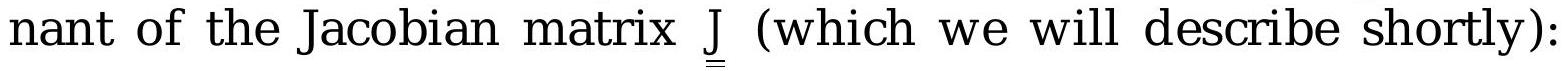
\includegraphics[max width=\textwidth]{2022_11_30_0cbb01a33d99487fc27fg-186}
\end{center}

$$
\begin{aligned}
& 1 \\
& \mathrm{z}^{2}
\end{aligned}
$$

\section{Superquadric Ellipsoids}
For the superquadric ellipsoids, the eight shells are centered at the origin, parameterized by " $r$ " for radius. In each octant of the $\mathrm{x}, \mathrm{y}, \mathrm{z}$ coordinate system, the superquadric shape is expressed via

$$
\begin{gathered}
\mathrm{x}(\mathrm{u}, \mathrm{v})=\pm \mathrm{ra}_{1} \cos (\mathrm{u})^{\mathrm{e}} \cos (\mathrm{v})^{\mathrm{n}}, \\
\mathrm{y}(\mathrm{u}, \mathrm{v})=\pm \mathrm{ra}_{2} \cos (\mathrm{v})^{\mathrm{n}} \sin (\mathrm{u})^{\mathrm{e}}, \\
\mathrm{z}(\mathrm{u}, \mathrm{v})=\pm \mathrm{ra}_{3} \sin (\mathrm{v})^{\mathrm{n}}, \\
0 \leq \mathrm{r} \leq 1, \quad 0 \leq \mathrm{v} \leq \pi / 2, \quad 0 \leq \mathrm{u} \leq \pi / 2 .
\end{gathered}
$$

Since the density is the same in each octant, we compute the integral in the first octant (where the signs are all positive) and multiply by eight. We need to compute the Jacobian determinant, multiply out $\mathrm{x}^{2}, \mathrm{y}^{2}$, and $\mathrm{z}^{2}$ in terms of $\sin$ and $\cos$, and then simplify using $\beta(~)$ functions. Our

\begin{center}
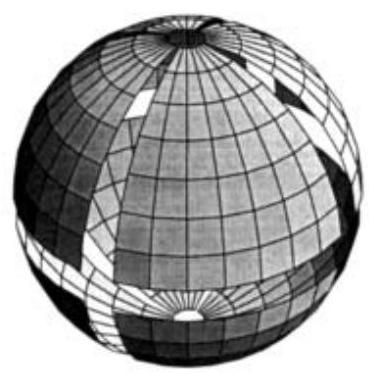
\includegraphics[max width=\textwidth]{2022_11_30_0cbb01a33d99487fc27fg-186(1)}
\end{center}

Figure 5. The eight octants for the superquadric ellipsoid. We integrate from the origin, where $r=0$, to the surface, where $r=1$.

\begin{center}
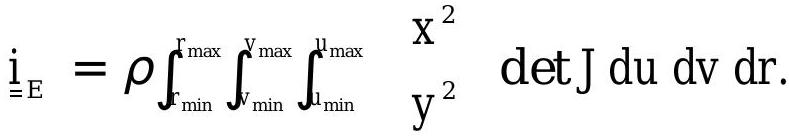
\includegraphics[max width=\textwidth]{2022_11_30_0cbb01a33d99487fc27fg-186(2)}
\end{center}

\section{III.8 RIGID PHYSICALLY BASED SUPERQUADRICS}
integration limits are from 0 to 1 for $r$, to get all of the "shells," and from 0 to $\pi / 2$ for the surface parameters:

$$
\dot{i}_{\mathrm{E}}=8 \rho \int_{0}^{1} \int_{0}^{\pi / 2} \int_{\mathrm{z}^{2}}^{\pi / 2} \mathrm{y}^{2} \operatorname{det} \mathrm{J} d u d v d r
$$

The Jacobian matrix is given by

$$
\underline{=}=\begin{array}{llll}
\partial \mathrm{x} / \partial \mathrm{u} & \partial \mathrm{x} / \partial \mathrm{v} & \partial \mathrm{x} / \partial \mathrm{r} \\
\partial \mathrm{y} / \partial \mathrm{u} & \partial \mathrm{y} / \partial \mathrm{v} & \partial \mathrm{y} / \partial \mathrm{r} \\
\partial \mathrm{z} / \partial \mathrm{u} & \partial \mathrm{z} / \partial \mathrm{v} & \partial \mathrm{z} / \partial \mathrm{r}
\end{array}
$$

I will spare the reader the expression for the matrix itself, but provide the expression for the determinant of the matrix. Symbolic derivatives can be computed using a symbolic manipulation program such as Mathematica (Wolfram, 1991). The determinant in the first octant is given by

$$
\operatorname{det} J=\mathrm{a}_{1} \mathrm{a}_{2} \mathrm{a}_{3} e n \mathrm{r}^{2} \cos (\mathrm{u})^{-1+\mathrm{e}} \cos (\mathrm{v})^{-1+2 n} \sin (u)^{-1+e} \sin (\mathrm{v})^{-1+\mathrm{n}} .
$$

Introducing the determinant into our equation for $\mathrm{i}_{\mathrm{E}}$ and expanding, we obtain

$$
\underline{i}_{\mathrm{E}}=8 \rho \delta_{0}^{1 / 2} \mathrm{~b}^{\pi / 2}
$$

$$
\begin{aligned}
& \mathrm{a}_{1} \mathrm{a}_{2} \mathrm{a}_{3} \mathrm{enr}^{2} \cos (u)^{-1+\mathrm{t}} \cos (\mathrm{v})^{-1+2 \mathrm{n}} \sin (u)^{-1+\mathrm{t}} \sin (\mathrm{v})^{-1+\mathrm{n}} \\
& \mathrm{a}_{1}^{3} \mathrm{a}_{2} \mathrm{a}_{3} \mathrm{enr}^{4} \cos (u)^{-1+3 \mathrm{e}} \cos (\mathrm{v})^{-1+4 \mathrm{n}} \sin (u)^{-1+e} \sin (\mathrm{v})^{-1+\mathrm{n}} \\
& a_{1} a_{2}^{3} a_{3} e n r^{4} \cos (u)^{-1+e} \cos (v)^{-1+4 n} \sin (u)^{-1+3 e} \sin (v)^{-1+n} d u d v d r \text {. } \\
& \mathrm{a}_{1} \mathrm{a}_{2} \mathrm{a}_{3}^{3} \mathrm{enr}^{4} \cos (u)^{-1+e} \cos (v)^{-1+2 \mathrm{n}} \sin (u)^{-1+\mathrm{e}} \sin (\mathrm{v})^{-1+3 \mathrm{n}} 
\end{aligned}
$$

\section{III.8 RIGID PHYSICALLY BASED SUPERQUADRICS}
Note that we have cosine and sine functions in the form mentioned in Appendix C. We can simplify the integral with respect to u using $\beta($ ) functions. Thus,

$$
\begin{aligned}
& \mathrm{a}_{1} \mathrm{a}_{2} \mathrm{a}_{3} e n r^{2} \cos (v)^{-1+2 n} \sin (v)^{-1+n} \beta \frac{e}{2}, \frac{e}{2} \\
& i_{-\mathrm{E}}=4 \rho \int_{0}^{1} \int_{0}^{\pi / 2} \mathrm{a}_{1}^{3} \mathrm{a}_{2} \mathrm{a}_{3} e n r^{4} \cos (v)^{-1+4 n} \sin (v)^{-1+n} \beta \frac{3 e}{2}, \frac{e}{2} \mathrm{a}_{1} \mathrm{a}_{2}^{3} \mathrm{a}_{3} e n r^{4} \cos (v)^{-1+4 n} \sin (v)^{-1+n} \beta \frac{e}{2}, \frac{3 e}{2} d v d r . \\
& \mathrm{a}_{1} \mathrm{a}_{2} \mathrm{a}_{3}^{3} \mathrm{enr}^{4} \cos (v)^{-1+2 n} \sin (v)^{-1+3 n} \beta \frac{e}{2}, \frac{e}{2}
\end{aligned}
$$

We also note that we can simplify the integral with respect to v using $\beta($ ) functions, so

$$
\begin{aligned}
& \mathrm{a}_{1} \mathrm{a}_{2} \mathrm{a}_{3} \mathrm{enr}^{2} \beta \frac{\mathrm{e}}{2}, \frac{\mathrm{e}}{2} \beta \mathrm{n}, \frac{\mathrm{n}}{2} \\
& i_{E}=2 \rho \int^{1} \mathrm{a}_{1}^{3} \mathrm{a}_{2} \mathrm{a}_{3} \mathrm{enr}^{4} \beta \frac{3 \mathrm{e}}{2}, \frac{\mathrm{e}}{2} \beta 2 \mathrm{n}, \frac{\mathrm{n}}{2} \\
& a_{1} a_{2}^{3} a_{3} e n r^{4} \beta \frac{e}{2}, \frac{3 e}{2} \beta \quad 2 n, \frac{n}{2} \\
& a_{1} a_{2} a_{3}^{3} \mathrm{enr}^{4} \beta \frac{\mathrm{e}}{2}, \frac{e}{2} \beta n, \frac{3 n}{2}
\end{aligned}
$$

dr.

Finally, we note that we can easily simplify the integral of $\mathrm{r}^{\mathrm{n}}$ with respect to $\mathrm{r}$ :

$$
\begin{aligned}
& \frac{2}{3} \mathrm{a}_{1} \mathrm{a}_{2} \mathrm{a}_{3} \text { en } \beta \frac{\mathrm{e}}{2}, \frac{\mathrm{e}}{2} \beta \mathrm{n}, \frac{\mathrm{n}}{2} \\
& \mathrm{i}_{\mathrm{E}}=\rho \\
& { }_{5}^{2} a_{1}^{3} a_{2} a_{3} \text { en } \beta \frac{3 e}{2}, \frac{e}{2} \beta \quad 2 n, \frac{n}{2} \\
& { }_{5}^{2} a_{1} a_{2} a_{3} \operatorname{en} \beta \frac{e}{2}, \frac{3 e}{2} \beta 2 n, \frac{n}{2} \\
& { }_{5}^{2} a_{1} a_{2} a_{3}^{3} \operatorname{en} \beta \frac{e}{2}, \frac{e}{2} \beta n, \frac{3 n}{2} 
\end{aligned}
$$

\section{III.8 RIGID PHYSICALLY BASED SUPERQUADRICS}
Then the four components of $\mathrm{i}_{E}$ (in other words $\rho \mathrm{V}_{E^{\prime}}, \mathrm{i}_{1 E^{\prime}}, \mathrm{i}_{2 \mathrm{E}}$, and $\mathrm{i}_{3 E}$ ) are used to produce the volume and inertia tensor of the superquadric ellipsoids, as shown in the section entitled "Inertia Tensor, Superquadric Ellipsoid."

\section{Superquadric Toroids}
The toroids are broken down similarly, into eight "outer" pieces and eight "inner" pieces. In the first octant, the outer piece is given by

$$
\begin{aligned}
&\mathrm{x}_{\text {outer }}=\mathrm{a}_{1} \cos (\mathrm{u})^{\mathrm{e}}\left(\alpha+\mathrm{r} \cos (\mathrm{v})^{\mathrm{n}}\right), \\
&\mathrm{y}_{\text {outer }}=\mathrm{a}_{2} \sin (\mathrm{u})^{\mathrm{e}}\left(\alpha+\mathrm{r} \cos (\mathrm{v})^{\mathrm{n}}\right), \\
&\mathrm{z}_{\text {outer }}=\mathrm{a}_{3} \mathrm{r} \sin (\mathrm{v})^{\mathrm{n}} .
\end{aligned}
$$

The inner piece is given by

$$
\begin{aligned}
&x_{\text {inner }}=a_{1} \cos (u)^{e}\left(\alpha-\mathrm{r} \cos (v)^{\mathrm{n}}\right), \\
&y_{\text {iner }}=a_{2} \sin (u)^{\mathrm{e}}\left(\alpha-\mathrm{r} \cos (v)^{\mathrm{n}}\right), \\
&z_{\text {iner }}=a_{3} \mathrm{r} \sin (v)^{\mathrm{n}} .
\end{aligned}
$$

\begin{center}
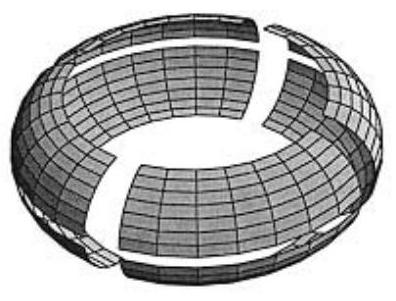
\includegraphics[max width=\textwidth]{2022_11_30_0cbb01a33d99487fc27fg-189}
\end{center}

(a)

\begin{center}
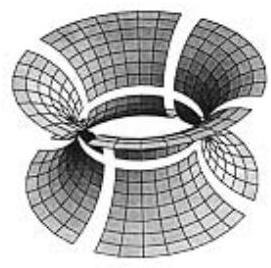
\includegraphics[max width=\textwidth]{2022_11_30_0cbb01a33d99487fc27fg-189(1)}
\end{center}

(b)

Figure 6 (a) The eight octants for the outer part of the superquadric toroid. We integrate from the torus centerline (not shown) where $r=0$ outwards to the surface, where $r=1$. (b) The eight octants for the inner part of the superquadric toroid. We integrate from the torus centerline (not shown) where $r=0$ inward to the surface, where $r=1$

\section{III.8 RIGID PHYSICALLY BASED SUPERQUADRICS}
where

$$
0 \leq \mathrm{r} \leq 1, \quad 0 \leq \mathrm{v} \leq \pi / 2, \quad 0 \leq u \leq \pi / 2 .
$$

We separately compute the Jacobian matrix, but we need to take the appropriate sign of the determinant of the outer and inner equations:

$$
\begin{aligned}
&\operatorname{det} J_{\text {outer }}=\mathrm{a}_{1} \mathrm{a}_{2} \mathrm{a}_{3} \text { enr } \cos (u)^{-1+e} \cos (v)^{-1+\mathrm{n}}\left(\alpha+\mathrm{r} \cos (v)^{\mathrm{n}}\right) \sin (u)^{-1+\mathrm{e}} \sin (v)^{-1+\mathrm{n}} \\
&\operatorname{det} \mathrm{J}_{\text {inner }}=-\mathrm{a}_{1} \mathrm{a}_{2} \mathrm{a}_{3} \text { enr } \cos (u)^{-1+e} \cos (v)^{-1+\mathrm{n}}\left(\alpha-\mathrm{r} \cos (v)^{\mathrm{n}}\right) \sin (u)^{-1+\mathrm{e}} \sin (v)^{-1+\mathrm{n}}
\end{aligned}
$$

We need to correctly combine the outer and inner parts into one integral, to obtain the expression for the four terms used in the expression for the inertia tensor of a superquadric toroid. Since the "inner" Jacobian matrix has the opposite handedness from the outer one, we need to change the sign on the determinant to maintain continuity at the common boundary between the two representations.

Thus, we let

$$
\begin{aligned}
& 1 \quad 1
\end{aligned}
$$

As before,

$$
\underline{i}_{\mathrm{T}} \equiv \begin{gathered}
\rho \mathrm{V}_{\mathrm{T}} \\
\mathrm{i}_{1 \mathrm{~T}} \\
\mathrm{i}_{2 \mathrm{~T}} \\
\mathrm{i}_{3 \mathrm{~T}}
\end{gathered} .
$$

\begin{center}
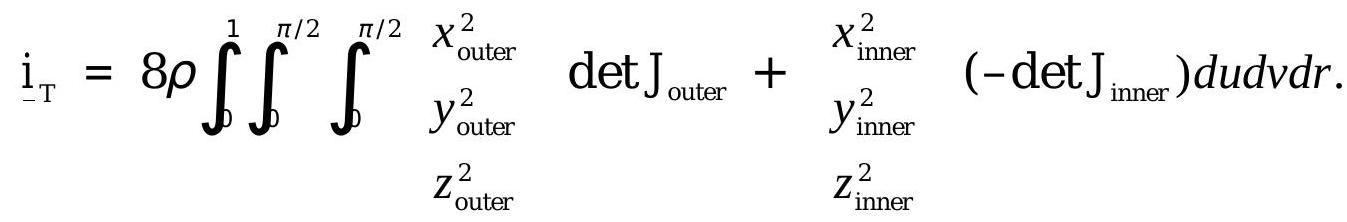
\includegraphics[max width=\textwidth]{2022_11_30_0cbb01a33d99487fc27fg-190}
\end{center}

\section{III.8 RIGID PHYSICALLY BASED SUPERQUADRICS}
The preceding integral expands to

$$
\begin{aligned}
& 2 \mathrm{a}_{1} \mathrm{a}_{2} \mathrm{a}_{3} \alpha \mathrm{enr} \cos (u)^{\mathrm{e}-1} \cos (\mathrm{v})^{\mathrm{n}-1} \sin (\mathrm{u})^{\mathrm{e}-1} \sin (\mathrm{v})^{\mathrm{n}-1} \\
& \underline{i}_{\mathrm{T}}=8 \rho \int_{0}^{1} \int_{0}^{\pi / 2} \int_{0}^{\pi / 2} 2 \mathrm{a}_{1}^{3} \mathrm{a}_{2} \mathrm{a}_{3} \alpha \operatorname{conr} \cos (u)^{3 \mathrm{e}-1} \cos (\mathrm{v})^{\mathrm{n}-1}\left(\alpha^{2}+3 \mathrm{a}^{2} \mathrm{a}_{2}^{3} \mathrm{a}_{3} \alpha \mathrm{cos}(\mathrm{v})^{2 \mathrm{n}}\right) \sin (u)^{\mathrm{e}-1} \sin (\mathrm{v})^{\mathrm{n}-1}(\mathrm{u})^{\mathrm{e}-1} \cos (\mathrm{v})^{\mathrm{n}-1}\left(\alpha^{2}+3 \mathrm{r}^{2} \cos (\mathrm{v})^{2 \mathrm{n}}\right) \sin (u)^{3 \mathrm{e}-1} \sin (\mathrm{v})^{\mathrm{n}-1} d u d v \\
& 2 \mathrm{a}_{1} \mathrm{a}_{2} \mathrm{a}_{3}^{3} \alpha e n r^{3} \cos (u)^{\mathrm{e}-1} \cos (\mathrm{v})^{\mathrm{n}-1} \sin (\mathrm{u})^{\mathrm{e}-1} \sin (\mathrm{v})^{3 \mathrm{n}-1}
\end{aligned}
$$

\section{and simplifies into $\beta($ ) functions}
$$
\begin{aligned}
& 2 \mathrm{a}_{1} \mathrm{a}_{2} \mathrm{a}_{3} \alpha \operatorname{en} \beta \frac{\mathrm{e}}{2}, \frac{\mathrm{e}}{2} \beta \frac{\mathrm{n}}{2}, \frac{\mathrm{n}}{2} \\
& \underline{i}_{\mathrm{T}}=\rho \\
& 2 \mathrm{a}_{1}^{3} \mathrm{a}_{2} \mathrm{a}_{3} \alpha^{3} \operatorname{en} \beta \frac{3 \mathrm{e}}{2}, \frac{\mathrm{e}}{2} \beta \frac{\mathrm{n}}{2}, \frac{\mathrm{n}}{2}+3 \mathrm{a}_{1}^{3} \mathrm{a}_{2} \mathrm{a}_{3} \alpha \operatorname{en} \beta \frac{3 \mathrm{e}}{2}, \frac{\mathrm{e}}{2} \beta \frac{3 \mathrm{n}}{2}, \frac{\mathrm{n}}{2} \\
& 2 \mathrm{a}_{1} \mathrm{a}_{2}^{3} \mathrm{a}_{3} \alpha^{3} \operatorname{en} \beta \frac{\mathrm{e}}{2}, \frac{3 \mathrm{e}}{2} \beta \frac{\mathrm{n}}{2}, \frac{\mathrm{n}}{2}+3 \mathrm{a}_{1} \mathrm{a}_{2}^{3} \mathrm{a}_{3} \alpha \operatorname{en} \beta \frac{\mathrm{e}}{2}, \frac{3 \mathrm{e}}{2} \beta \frac{3 \mathrm{n}}{2}, \frac{\mathrm{n}}{2} \\
& \mathrm{a}_{1} \mathrm{a}_{2} \mathrm{a}_{3}^{3} \alpha \mathrm{en} \beta \frac{\mathrm{e}}{2}, \frac{\mathrm{e}}{2} \beta \frac{\mathrm{n}}{2}, \frac{3 \mathrm{n}}{2}
\end{aligned}
$$

Then the four components of $\underline{i}_{T}$ (in other words $\rho V_{T}, i_{1 T}, i_{2 T}$, and $i_{3 T}$ ) are used to produce the volume and inertia tensor of the toroids.\\

\includegraphics[max width=\textwidth, center]{2022_11_30_0cbb01a33d99487fc27fg-194}

$$
\begin{gathered}
\text { 2-D GEOMETRY } \\
\text { AND } \\
\text { ALGORITHMS }
\end{gathered}
$$

\begin{center}
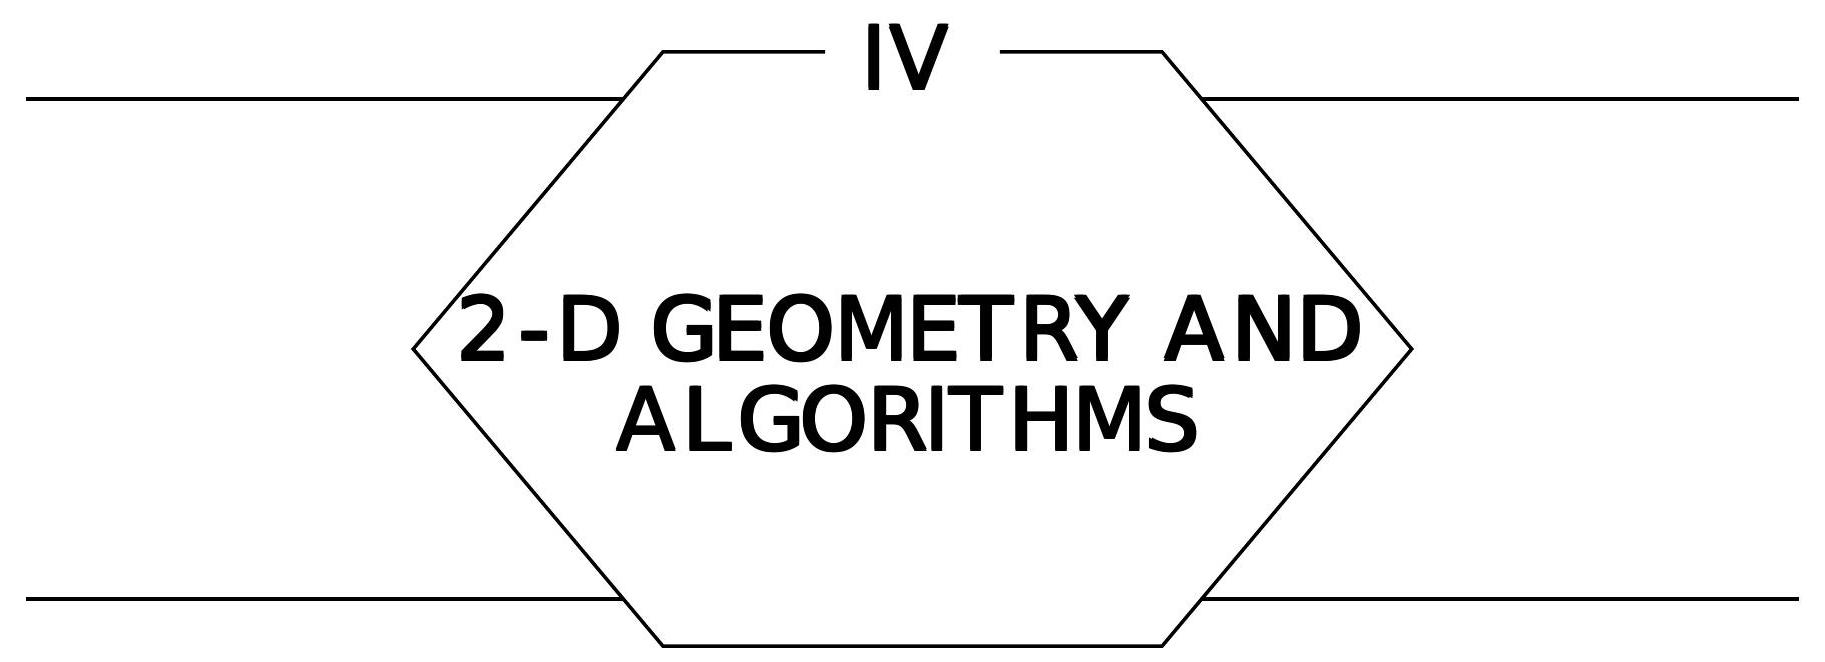
\includegraphics[max width=\textwidth]{2022_11_30_0cbb01a33d99487fc27fg-195}
\end{center}

Two-dimensional geometry is an important part of computer graphics. Figure-making, layout of geometric figures on a sheet, and projective geometry are examples of common applications. The Gems in this section focus on techniques for making pictures from two-dimensional entities.

The first, third, and fifth Gems deal with methods of drawing various two-dimensional curves. The first Gem describes how to draw elliptical arcs. The third Gem discusses an efficient technique for circle clipping. The fifth Gem provides a recipe for generating circular arc fillets between two lines.

The second Gem describes techniques for producing well organized figures, helping with the related problems of where to place items and how to connect them.

The fourth, sixth, and seventh Gems present clever improvements upon previous Gems. The fourth and sixth Gems discuss efficient computation of the intersection between two lines, while the seventh Gem discusses the construction of circles tangent to other figures, and related problems.\\
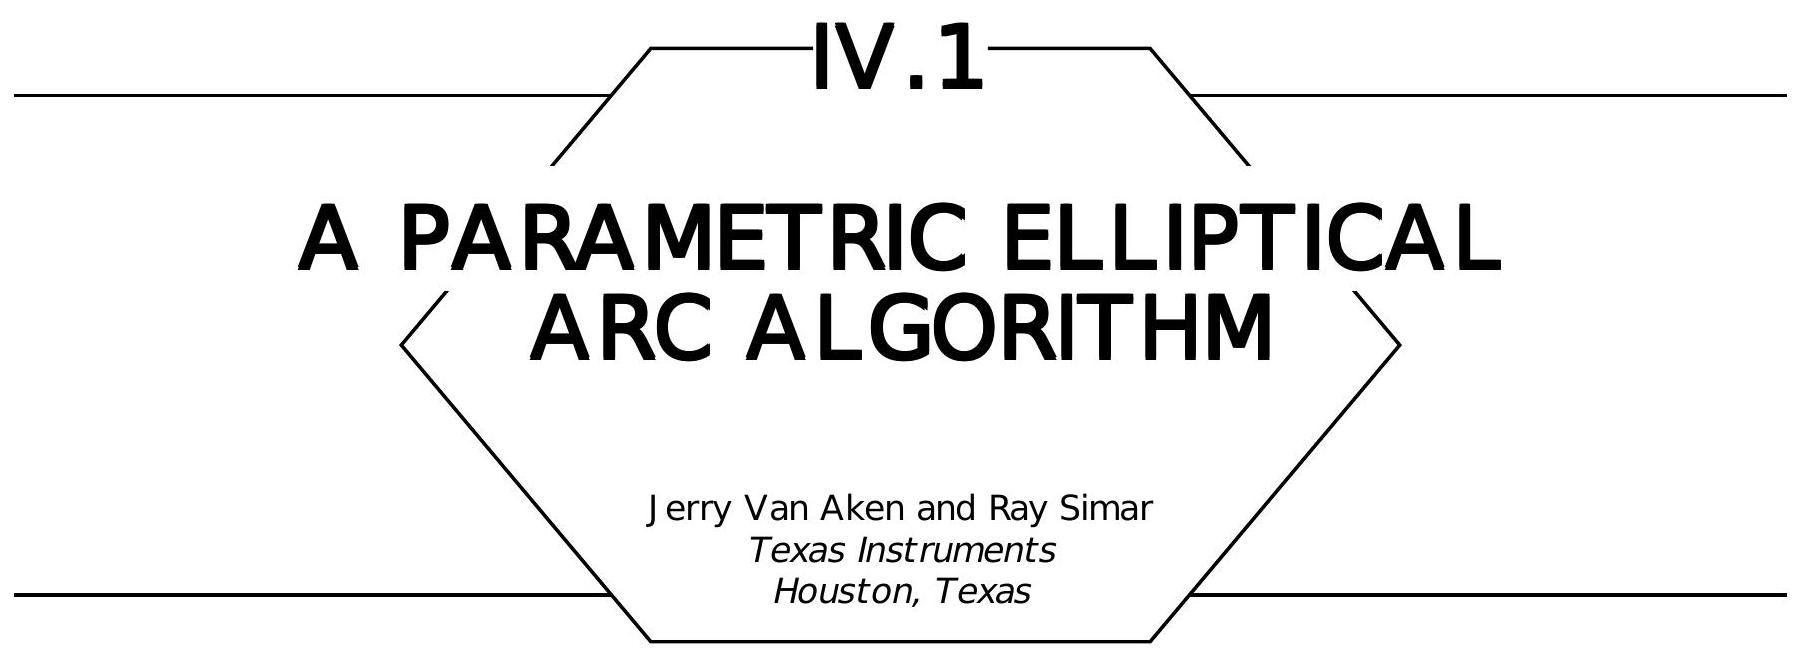
\includegraphics[max width=\textwidth, center]{2022_11_30_0cbb01a33d99487fc27fg-196}

Sometimes an arc of a circle or of an ellipse is a better choice than a cubic spline for representing a particular curved shape. Because circles and ellipses are inherently simpler curves than cubics, the algorithms for generating them should also be simpler. This is chiefly why conic splines are popular in applications such as the generation of font outlines, where drawing speed is of critical importance.

This note describes an algorithm for generating points along an elliptical arc. The points are separated by a fixed angular increment specified in radians of elliptical arc. The algorithm is based on a parametric representation of the ellipse. It is particularly inexpensive in terms of the amount of computation required. Only a few integer (or fixed-point) shifts, additions, and subtractions are needed to generate each point-without compromising accuracy.

\section{The Algorithm}
The QtrElips function in Fig. 1 is a version of the algorithm that uses floating-point operations. An integer-only version is presented later. The first six arguments to the function are the $\mathrm{x}$ and $\mathrm{y}$ coordinates of the vertices $\mathrm{P}, \mathrm{Q}$, and $\mathrm{K}$ of a control polygon (a triangle) that defines the curve. The arc beings at $P$, ends at $Q$, and is completely contained within the triangle formed by the three points. The last argument, $\Delta t$, specifies the (approximate) angular increment in radians between successive points plotted along the curve. This argument is a fractional value in the range $1 \geq \Delta t>0$.
